% !TeX spellcheck = russian-aot-ieyo
% Зачем: Определяет класс документа (То, как будет выглядеть документ)
% Примечание: параметр draft помечает строки, вышедшие за границы страницы, прямоугольником, в фильной версии его нужно удалить.
\documentclass[a4paper,14pt,russian,oneside,final]{extreport}

% Зачем: Настройка Times New Roman.
% Рекомендовано для Windows (нужен PSCyr, подробности см. в fonts_windows.tex)
% раскомментировать, чтобы использовать:
% Зачем: Предоставляет проприетарный Times New Roman.
% ОБНОВЛЕНИЕ: лучше использовать scalable-cyrfonts-tex: меньше проблем с установкой
% Из руководства к PSCyr: "Во избежание проблем пакет PSCyr должен загружаться перед пакета-ми inputenc и babel".
% Примечание: Требует шаманства при установке, инструкция http://plumbum-blog.blogspot.com/2010/06/miktex-28-pscyr-04d.html
% http://blog.harrix.org/?p=444
\usepackage{pscyr}

% Зачем: Выбор внутренней TeX кодировки.
\usepackage[T2A]{fontenc}

% не забудьте закомментировать \input{fonts_linux}

% Рекомендовано для Linux (нужен scalable-cyrfonts-tex, подробности см. в fonts_linux.tex)
% раскомментировать, чтобы использовать:
%\input{fonts_linux}% не забудьте закомментировать % Зачем: Предоставляет проприетарный Times New Roman.
% ОБНОВЛЕНИЕ: лучше использовать scalable-cyrfonts-tex: меньше проблем с установкой
% Из руководства к PSCyr: "Во избежание проблем пакет PSCyr должен загружаться перед пакета-ми inputenc и babel".
% Примечание: Требует шаманства при установке, инструкция http://plumbum-blog.blogspot.com/2010/06/miktex-28-pscyr-04d.html
% http://blog.harrix.org/?p=444
\usepackage{pscyr}

% Зачем: Выбор внутренней TeX кодировки.
\usepackage[T2A]{fontenc}



% Зачем: Установка кодировки исходных файлов.
\usepackage[utf8]{inputenc}

% Зачем: Делает результирующий PDF "searchable and copyable".
\usepackage{cmap}

% Зачем: Чтобы можно было использовать русские буквы в формулах, но в случае использования предупреждать об этом.
\usepackage[warn]{mathtext}

% Зачем: Учет особенностей различных языков.
\usepackage[russian]{babel}

% Зачем: Добавляет поддержу дополнительных размеров текста 8pt, 9pt, 10pt, 11pt, 12pt, 14pt, 17pt, and 20pt.
% Почему: Пункт 2.1.1 Требований по оформлению пояснительной записки.
\usepackage{extsizes}


% Зачем: Длинна, пимерно соответвующая 5 символам
% Почему: Требования содержат странное требование про отсупы в 5 символов (для немоноширинного шрифта :| )
\newlength{\fivecharsapprox}
\setlength{\fivecharsapprox}{6ex}


% Зачем: Добавляет отступы для абзацев.
% Почему: Пункт 2.1.3 Требований по оформлению пояснительной записки.
\usepackage{indentfirst}
\setlength{\parindent}{\fivecharsapprox} % Примерно соответсвует 5 символам.


% Зачем: Настраивает отступы от границ страницы.
% Почему: Пункт 2.1.2 Требований по оформлению пояснительной записки.
\usepackage[left=3cm,top=2.0cm,right=1.5cm,bottom=2.7cm]{geometry}


% Зачем: Настраивает межстрочный интервал, для размещения 40 +/- 3 строки текста на странице.
% Почему: Пункт 2.1.1 Требований по оформлению пояснительной записки.
\usepackage[nodisplayskipstretch]{setspace} 
\setstretch{1.1}
%\onehalfspacing

% Зачем: Выбор шрифта по-умолчанию. 
% Почему: Пункт 2.1.1 Требований по оформлению пояснительной записки.
% Примечание: В требованиях не указан, какой именно шрифт использовать. По традиции используем TNR.
\renewcommand{\rmdefault}{ftm} % Times New Roman


% Зачем: Отключает использование изменяемых межсловных пробелов.
% Почему: Так не принято делать в текстах на русском языке.
\frenchspacing


% Зачем: Сброс счетчика сносок для каждой страницы
% Примечание: в "Требованиях по оформлению пояснительной записки" не указано, как нужно делать, но в других БГУИРовских докуметах рекомендуется нумерация отдельная для каждой страницы
\usepackage{perpage}
\MakePerPage{footnote}


% Зачем: Добавляет скобку 1) к номеру сноски
% Почему: Пункты 2.9.2 и 2.9.1 Требований по оформлению пояснительной записки.
\makeatletter 
\def\@makefnmark{\hbox{\@textsuperscript{\normalfont\@thefnmark)}}}
\makeatother


% Зачем: Расположение сносок внизу страницы
% Почему: Пункт 2.9.2 Требований по оформлению пояснительной записки.
\usepackage[bottom]{footmisc}


% Зачем: Переопределяем стандартную нумерацию, т.к. в отчете будут только section и т.д. в терминологии TeX
\makeatletter
\renewcommand{\thesection}{\arabic{section}}
\makeatother


% Зачем: Пункты (в терминологии требований) в терминологии TeX subsubsection должны нумероваться
% Почему: Пункт 2.2.3 Требований по оформлению пояснительной записки.
\setcounter{secnumdepth}{3}


% Зачем: Настраивает отступ между таблицей с содержанимем и словом СОДЕРЖАНИЕ
% Почему: Пункт 2.2.7 Требований по оформлению пояснительной записки.
\usepackage{tocloft}
\setlength{\cftbeforetoctitleskip}{-1em}
\setlength{\cftaftertoctitleskip}{1em}


% Зачем: Определяет отступы слева для записей в таблице содержания.
% Почему: Пункт 2.2.7 Требований по оформлению пояснительной записки.
\makeatletter
\renewcommand{\l@section}{\@dottedtocline{1}{0.5em}{1.2em}}
\renewcommand{\l@subsection}{\@dottedtocline{2}{1.7em}{2.0em}}
\makeatother


% Зачем: Работа с колонтитулами
\usepackage{fancyhdr} % пакет для установки колонтитулов
\pagestyle{fancy} % смена стиля оформления страниц


% Зачем: Нумерация страниц располагается справа снизу страницы
% Почему: Пункт 2.2.8 Требований по оформлению пояснительной записки.
\fancyhf{} % очистка текущих значений
\fancyfoot[R]{\thepage} % установка верхнего колонтитула
\renewcommand{\footrulewidth}{0pt} % убрать разделительную линию внизу страницы
\renewcommand{\headrulewidth}{0pt} % убрать разделительную линию вверху страницы
\fancypagestyle{plain}{ 
    \fancyhf{}
    \rfoot{\thepage}}


% Зачем: Задает стиль заголовков раздела жирным шрифтом, прописными буквами, без точки в конце
% Почему: Пункты 2.1.1, 2.2.5, 2.2.6 и ПРИЛОЖЕНИЕ Л Требований по оформлению пояснительной записки.
\makeatletter
\renewcommand\section{%
  \clearpage\@startsection {section}{1}%
    {\fivecharsapprox}%
    {-1em \@plus -1ex \@minus -.2ex}%
    {1em \@plus .2ex}%
    {\raggedright\hyphenpenalty=10000\normalfont\large\bfseries\MakeUppercase}}
\makeatother


% Зачем: Задает стиль заголовков подразделов
% Почему: Пункты 2.1.1, 2.2.5 и ПРИЛОЖЕНИЕ Л Требований по оформлению пояснительной записки.
\makeatletter
\renewcommand\subsection{%
  \@startsection{subsection}{2}%
    {\fivecharsapprox}%
    {-1em \@plus -1ex \@minus -.2ex}%
    {1em \@plus .2ex}%
    {\raggedright\hyphenpenalty=10000\normalfont\normalsize\bfseries}}
\makeatother


% Зачем: Задает стиль заголовков пунктов
% Почему: Пункты 2.1.1, 2.2.5 и ПРИЛОЖЕНИЕ Л Требований по оформлению пояснительной записки.
\makeatletter
\renewcommand\subsubsection{
  \@startsection{subsubsection}{3}%
    {\fivecharsapprox}%
    {-1em \@plus -1ex \@minus -.2ex}%
    {\z@}%
    {\raggedright\hyphenpenalty=10000\normalfont\normalsize\bfseries}}
\makeatother

% Зачем: для оформления введения и заключения, они должны быть выровнены по центру.
% Почему: Пункты 1.1.15 и 1.1.11 Требований по оформлению пояснительной записки.
\makeatletter
\newcommand\sectioncentered{%
  \clearpage\@startsection {section}{1}%
    {\z@}%
    {-1em \@plus -1ex \@minus -.2ex}%
    {1em \@plus .2ex}%
    {\centering\hyphenpenalty=10000\normalfont\large\bfseries\MakeUppercase}%
    }
\makeatother



% Зачем: Задает стиль библиографии
% Почему: Пункт 2.8.6 Требований по оформлению пояснительной записки.
\bibliographystyle{styles/belarus-specific-utf8gost780u}


% Зачем: Пакет для вставки картинок
% Примечание: Объяснение, зачем final - http://tex.stackexchange.com/questions/11004/why-does-the-image-not-appear
\usepackage[final]{graphicx}
\DeclareGraphicsExtensions{.pdf,.png,.jpg,.eps}


% Зачем: Директория в которой будет происходить поиск картинок
\graphicspath{{figures/}}


% Зачем: Добавление подписей к рисункам
\usepackage[nooneline]{caption}
\usepackage{subcaption}

% Зачем: чтобы работала \No в новых латехах
\DeclareRobustCommand{\No}{\ifmmode{\nfss@text{\textnumero}}\else\textnumero\fi}

% Зачем: поворот ячеек таблиц на 90 градусов
\usepackage{rotating}
\DeclareRobustCommand{\povernut}[1]{\begin{sideways}{#1}\end{sideways}}


% Зачем: когда в формулах много кириллических символов команда \text{} занимает много места
\DeclareRobustCommand{\x}[1]{\text{#1}}


% Зачем: Задание подписей, разделителя и нумерации частей рисунков
% Почему: Пункт 2.5.5 Требований по оформлению пояснительной записки.
\DeclareCaptionLabelFormat{stbfigure}{Рисунок #2}
\DeclareCaptionLabelFormat{stbtable}{Таблица #2}
\DeclareCaptionLabelSeparator{stb}{~--~}
\captionsetup{labelsep=stb}
\captionsetup[figure]{labelformat=stbfigure,justification=centering}
\captionsetup[table]{labelformat=stbtable,justification=raggedright}
\renewcommand{\thesubfigure}{\asbuk{subfigure}}

% Зачем: Окружения для оформления формул
% Почему: Пункт 2.4.7 требований по оформлению пояснительной записки и специфические требования различных кафедр
% Пример использования смотри в course_content.tex, строка 5
\usepackage{calc}
\newlength{\lengthWordWhere}
\settowidth{\lengthWordWhere}{где}
\newenvironment{explanationx}
    {%
    %%% Следующие строки определяют специфические требования разных редакций стандартов. Раскоменнтируйте нужную строку
    %% стандартный абзац, СТП-01 2010
    %\begin{itemize}[leftmargin=0cm, itemindent=\parindent + \lengthWordWhere + \labelsep, labelsep=\labelsep]
    %% без отступа, СТП-01 2013
    \begin{itemize}[leftmargin=0cm, itemindent=\lengthWordWhere + \labelsep , labelsep=\labelsep]%
    \renewcommand\labelitemi{}%
    }
    {%
    %\\[\parsep]
    \end{itemize}
    }

% Старое окружение для "где". Сохранено для совместимости
\usepackage{tabularx}

\newenvironment{explanation}
    {
    %%% Следующие строки определяют специфические требования разных редакций стандартов. Раскоменнтируйте нужные 2 строки
    %% стандартный абзац, СТП-01 2010
    %\par 
    %\tabularx{\textwidth-\fivecharsapprox}{@{}ll@{ --- } X }
    %% без отступа, СТП-01 2013
    \noindent 
    \tabularx{\textwidth}{@{}ll@{ --- } X }
    }
    { 
    \\[\parsep]
    \endtabularx
    }


% Зачем: Удобная вёрстка многострочных формул, масштабирующийся текст в формулах, формулы в рамках и др
\usepackage{amsmath}


% Зачем: Поддержка ажурного и готического шрифтов 
\usepackage{amsfonts}


% Зачем: amsfonts + несколько сотен дополнительных математических символов
\usepackage{amssymb}


% Зачем: Окружения «теорема», «лемма»
\usepackage{amsthm}


% Зачем: Производить арифметические операции во время компиляции TeX файла
\usepackage{calc}

% Зачем: Производить арифметические операции во время компиляции TeX файла
\usepackage{fp}

% Зачем: Пакет для работы с перечислениями
\usepackage{enumitem}
\makeatletter
 \AddEnumerateCounter{\asbuk}{\@asbuk}{щ)}
\makeatother


% Зачем: Устанавливает символ начала простого перечисления
% Почему: Пункт 2.3.5 Требований по оформлению пояснительной записки.
\setlist{nolistsep}


% Зачем: Устанавливает символ начала именованного перечисления
% Почему: Пункт 2.3.8 Требований по оформлению пояснительной записки.
\renewcommand{\labelenumi}{\asbuk{enumi})}
\renewcommand{\labelenumii}{\arabic{enumii})}

% Зачем: Устанавливает отступ от границы документа до символа списка, чтобы этот отступ равнялся отступу параграфа
% Почему: Пункт 2.3.5 Требований по оформлению пояснительной записки.

\setlist[itemize,0]{itemindent=\parindent + 2.2ex,leftmargin=0ex,label=--}
\setlist[enumerate,1]{itemindent=\parindent + 2.7ex,leftmargin=0ex}
\setlist[enumerate,2]{itemindent=\parindent + \parindent - 2.7ex}

% Зачем: Включение номера раздела в номер формулы. Нумерация формул внутри раздела.
\AtBeginDocument{\numberwithin{equation}{section}}

% Зачем: Включение номера раздела в номер таблицы. Нумерация таблиц внутри раздела.
\AtBeginDocument{\numberwithin{table}{section}}

% Зачем: Включение номера раздела в номер рисунка. Нумерация рисунков внутри раздела.
\AtBeginDocument{\numberwithin{figure}{section}}


% Зачем: Дополнительные возможности в форматировании таблиц
\usepackage{makecell}
\usepackage{multirow}
\usepackage{array}


% Зачем: "Умная" запятая в математических формулах. В дробных числах не добавляет пробел
% Почему: В требованиях не нашел, но в русском языке для дробных чисел используется {,} а не {.}
\usepackage{icomma}

% Зачем: макрос для печати римских чисел
\makeatletter
\newcommand{\rmnum}[1]{\romannumeral #1}
\newcommand{\Rmnum}[1]{\expandafter\@slowromancap\romannumeral #1@}
\makeatother


% Зачем: Управление выводом чисел.
\usepackage{sistyle}
\SIdecimalsign{,}

% Зачем: inline-коментирование содержимого.
\newcommand{\ignore}[2]{\hspace{0in}#2}


% Зачем: Возможность коментировать большие участки документа
\usepackage{verbatim}


\usepackage{xcolor}


% Зачем: Оформление листингов кода
% Примечание: final нужен для переопределения режима draft, в котором листинги не выводятся в документ.
\usepackage[final]{listings}


% Зачем: настройка оформления листинга для языка F#
\definecolor{bluekeywords}{rgb}{0.13,0.13,1}
\definecolor{greencomments}{rgb}{0,0.5,0}
\definecolor{turqusnumbers}{rgb}{0.17,0.57,0.69}
\definecolor{redstrings}{rgb}{0.5,0,0}

\renewcommand{\lstlistingname}{Листинг}

\lstdefinelanguage{FSharp}
    {morekeywords={abstract,and,as,assert,base,begin,class,default,delegate,do,done,downcast,downto,elif,else,end,exception,extern,false,finally,for,fun,function,global,if,in,inherit,inline,interface,internal,lazy,let,let!,match,member,module,mutable,namespace,new,not,null,of,open,or,override,private,public,rec,return,return!,select,static,struct,then,to,true,try,type,upcast,use,use!,val,void,when,while,with,yield,yield!,asr,land,lor,lsl,lsr,lxor,mod,sig,atomic,break,checked,component,const,constraint,constructor,continue,eager,event,external,fixed,functor,include,method,mixin,object,parallel,process,protected,pure,sealed,tailcall,trait,virtual,volatile},
    keywordstyle=\bfseries\color{bluekeywords},
    sensitive=false,
    morecomment=[l][\color{greencomments}]{///},
    morecomment=[l][\color{greencomments}]{//},
    morecomment=[s][\color{greencomments}]{{(*}{*)}},
    morestring=[b]",
    stringstyle=\color{redstrings},
    }

\lstdefinestyle{fsharpstyle}{
   xleftmargin=0ex,
   language=FSharp,
   basicstyle=\footnotesize\ttfamily,
   breaklines=true,
   columns=fullflexible
}

\lstdefinestyle{csharpinlinestyle} {
  language=[Sharp]C,
  morekeywords={yield,var,get,set,from,select,partial,where,async,await},
  breaklines=true,
  columns=fullflexible,
  basicstyle=\footnotesize\ttfamily
}

\lstdefinestyle{csharpstyle}{
  language=[Sharp]C,
  frame=lr,
  rulecolor=\color{blue!80!black}}

\lstset{style=fsharpstyle}  

% Зачем: Нумерация листингов в пределах секции
\AtBeginDocument{\numberwithin{lstlisting}{section}}

\usepackage[normalem]{ulem}

\usepackage[final,hidelinks]{hyperref}
% Моноширинный шрифт выглядит визуально больше, чем пропорциональный шрифт, если их размеры одинаковы. Искусственно уменьшаем размер ссылок.
\renewcommand{\UrlFont}{\small\rmfamily\tt}

\usepackage[square,numbers,sort&compress]{natbib}
\setlength{\bibsep}{0em}

% Магия для подсчета разнообразных объектов в документе
\usepackage{lastpage}
\usepackage{totcount}
\regtotcounter{section}

\usepackage{etoolbox}

\newcounter{totfigures}
\newcounter{tottables}
\newcounter{totreferences}
\newcounter{totequation}

\providecommand\totfig{} 
\providecommand\tottab{}
\providecommand\totref{}
\providecommand\toteq{}

\makeatletter
\AtEndDocument{%
  \addtocounter{totfigures}{\value{figure}}%
  \addtocounter{tottables}{\value{table}}%
  \addtocounter{totequation}{\value{equation}}
  \immediate\write\@mainaux{%
    \string\gdef\string\totfig{\number\value{totfigures}}%
    \string\gdef\string\tottab{\number\value{tottables}}%
    \string\gdef\string\totref{\number\value{totreferences}}%
    \string\gdef\string\toteq{\number\value{totequation}}%
  }%
}
\makeatother

\pretocmd{\section}{\addtocounter{totfigures}{\value{figure}}\setcounter{figure}{0}}{}{}
\pretocmd{\section}{\addtocounter{tottables}{\value{table}}\setcounter{table}{0}}{}{}
\pretocmd{\section}{\addtocounter{totequation}{\value{equation}}\setcounter{equation}{0}}{}{}
\pretocmd{\bibitem}{\addtocounter{totreferences}{1}}{}{}



% Для оформления таблиц не влязящих на 1 страницу
\usepackage{longtable}

% Для включения pdf документов в результирующий файл
\usepackage{pdfpages}

% Для использования знака градуса и других знаков
% http://ctan.org/pkg/gensymb
\usepackage{gensymb}

% Зачем: преобразовывать текст в верхний регистр командой MakeTextUppercase
\usepackage{textcase}

% Зачем: Переносы в словах с тире.
% Тире в словае заменяем на \hyph: аппаратно\hyphпрограммный.
% https://stackoverflow.com/questions/2193307/how-to-get-latex-to-hyphenate-a-word-that-contains-a-dash#
\def\hyph{-\penalty0\hskip0pt\relax}

% Добавляем абзацный отступ для библиографии
% https://github.com/mstyura/bsuir-diploma-latex/issues/19
\setlength\bibindent{-1.0900cm}

\makeatletter
\renewcommand\NAT@bibsetnum[1]{\settowidth\labelwidth{\@biblabel{#1}}%
   \setlength{\leftmargin}{\bibindent}\addtolength{\leftmargin}{\dimexpr\labelwidth+\labelsep\relax}%
   \setlength{\itemindent}{-\bibindent+\fivecharsapprox-0.240cm}%
   \setlength{\listparindent}{\itemindent}
\setlength{\itemsep}{\bibsep}\setlength{\parsep}{\z@}%
   \ifNAT@openbib
     \addtolength{\leftmargin}{\bibindent}%
     \setlength{\itemindent}{-\bibindent}%
     \setlength{\listparindent}{\itemindent}%
     \setlength{\parsep}{10pt}%
   \fi
}



\newcommand{\csharp}{C\#}
\newcommand{\cpp}{C\texttt{\hspace{-0.3ex}+\hspace{-0.25ex}+}}
\newcommand{\dotnet}{Microsoft .NET}
\newcommand{\netfx}{.NET Framework}
\newcommand{\java}{Java}
\newcommand{\unity}{Unity}
\newcommand{\diploma}{Программный модуль для расчёта траектории движения объектов в игровых приложениях}
\newcommand{\diplomabig}{ПРОГРАММНЫЙ МОДУЛЬ ДЛЯ РАСЧЁТА ТРАЕКТОРИИ ДВИЖЕНИЯ ОБЪЕКТОВ В ИГРОВЫХ ПРИЛОЖЕНИЯХ}

\begin{document}

\begin{titlepage}
  \begin{center}
    Министерство образования Республики Беларусь\\[1em]
    Учреждение образования\\
    БЕЛОРУССКИЙ ГОСУДАРСТВЕННЫЙ УНИВЕРСИТЕТ \\
    ИНФОРМАТИКИ И РАДИОЭЛЕКТРОНИКИ\\[1em]

    \begin{minipage}{\textwidth}
      \begin{flushleft}
        \begin{tabular}{ l l }
          Факультет & Компьютерных систем и сетей\\
          Кафедра   & Информатики
        \end{tabular}
      \end{flushleft}
    \end{minipage}\\[1em]

    \begin{flushright}
      \begin{minipage}{0.4\textwidth}
        \textit{К защите допустить:}\\[0.8em]
        Заведующая кафедрой информатики\\[0.45em]
        \underline{\hspace*{2.8cm}} Н.А. Волорова
      \end{minipage}\\[2.2em]
    \end{flushright}

    %%
    %% ВНИМАНИЕ: на некторых факультетах (ФКП) и кафедрах (ПИКС) слова "ПОЯСНИТЕЛЬНАЯ ЗАПИСКА" предлагается (требуется) оформлять полужирным начертанием. Раскомментируйте нужную для вас строку:
    %%
    %\textbf{ПОЯСНИТЕЛЬНАЯ ЗАПИСКА}\\
    {ПОЯСНИТЕЛЬНАЯ ЗАПИСКА}\\
    {к дипломному проекту}\\
    {на тему:}\\[1em]
    \textbf{\large \diplomabig}\\[1em]


    {БГУИР ДП 1-40 04 01 00 026 ПЗ}\\[2em]
    
    \begin{tabular}{ p{0.65\textwidth}p{0.25\textwidth} }
      Студент & А.А. Глотов \\
      Руководитель & Е.В. Кукар \\
      Консультанты: &\\
      \hspace*{3ex}\emph{от кафедры информатики} & А.А. Волосевич \\
      \hspace*{3ex}\emph{по экономической части} & Т.Е. Наганова \\
      %%
      %% ВНИМАНИЕ: в зависимости от выбранной темы, у вас консультант может быть как по охране труда, так и по:
        % экологической безопасности
        % ресурсосбережению
        % энергосбережению
      %%
      %% Впишите правильную формулировку по необходимости
      Нормоконтролёр & Н.Н. Бабенко \\
      
      Рецензент &
    \end{tabular}
    
    \vfill
    {\normalsize Минск 2020}
  \end{center}
\end{titlepage}
 % page 1

\sectioncentered*{Реферат}
\thispagestyle{empty}
%%
%% ВНИМАНИЕ: этот реферат не соответствует СТП-01 2013
%% пример оформления реферата смотрите здесь: http://www.bsuir.by/m/12_100229_1_91132.docx 
%%

\begin{center}
Пояснительная записка \pageref*{LastPage}~с., \totfig{}~рис., \tottab{}~табл., \totref{}~источников.
\diplomabig	
\end{center}

\textbf{Ключевые слова}: построение траектории движения объектов; физические игровые движки; игровой движок Unity; моедлирование поведения игровых объектов.

\textbf{Объект проектирования:} программный модуль для вычисления и построения траектории движения игровых объектов.

\textbf{Цель проектирования}: разработка программного модуля для расчета и построения траектории движения в игровых приложениях.

Проведен анализ различных физических игровых движков. Рассмотрены математические модели построения траектории движения объектов. Рассмотрены различные физические движки и их возможности. 

Создан программный модуль с использованием среды разработки Unity и физического движка PhysX и программный модуль с использованием фреймворка libGDX и физического движка Box2D для построения траектории движения объектов в двумерном пространстве. Проведен анализ полученных модулей, описаны положительные и отрицательные стороны каждого из них. 

Создан программный модуль с использованием среды разработки Unity и физического движка PhysX для построения траектории движения объектов в трехмерном пространстве.

В разделе технико-экономического обоснования был произведён расчёт затрат на создание ПО, а также прибыли от разработки, получаемой разработчиком.

Проведенные расчеты показали экономическую целесообразность проекта.
\clearpage
 % page 2

{
  \newgeometry{top=1.25cm,bottom=1.25cm,right=1cm,left=2cm,twoside}
  \thispagestyle{empty}
  \setlength{\parindent}{0em}

  \newcommand{\lineunderscore}{\uline{\hspace*{\fill}}}

  \begin{center}
    Министерство образования Республики Беларусь\\
    Учреждение образования\\
    БЕЛОРУССКИЙ ГОСУДАРСТВЕННЫЙ УНИВЕРСИТЕТ \\
    ИНФОРМАТИКИ И РАДИОЭЛЕКТРОНИКИ\\[1em]
  

  \begin{minipage}{\textwidth}
    \begin{flushleft}
      \begin{tabular}{ p{0.20\textwidth}p{0.31\textwidth}p{0.20\textwidth}p{0.20\textwidth} @{} }
        Факультет & КСиС & Кафедра & Информатики \\
        Специальность   & 1-40 04 01 & Специализация & 00
      \end{tabular}
    \end{flushleft}
  \end{minipage}\\[1em]

  \begin{minipage}{\textwidth}
    \begin{flushright}
      \begin{tabular}{p{0.40\textwidth}}
        УТВЕРЖДАЮ \\[0.5em]
        \underline{\hspace*{7em}} Н.А. Волорова \\
        <<\underline{\hspace*{4ex}}>> \underline{\hspace*{7em}} 2020 г.
      \end{tabular}
    \end{flushright}
  \end{minipage}\\[1em]

  \textbf{ЗАДАНИЕ} \\
  \textbf{по дипломному проекту студента}

  
  \lineunderscore\uline{Глотова Артёма Алексеевича}\lineunderscore \\
  {\small (фамилия, имя, отчество) }

  \end{center}

  1. Тема проекта:
  \uline{Программный модуль для расчёта траектории движения объектов в игровых приложениях}\lineunderscore
  \lineunderscore\\
  \lineunderscore\\
  утверждена приказом по университету от \uline{\hspace*{1.5em}} \uline{\hspace*{5em}} 2013 г.  \No{} \uline{\hspace*{2em}}-с

  \vspace{1em}

  2. Срок сдачи студентом законченного проекта (работы): \lineunderscore

  \vspace{1em}

  3. Исходные данные к проекту (работе):
  \uline{Тип операционной системы - ОС Windows 10; Языки программирования: С\#, Kotlin}\lineunderscore
  \lineunderscore\\
  \lineunderscore\\
  \lineunderscore\\
  \lineunderscore

  \vspace{1em}

  4. Содержание пояснительной записки (перечень подлежащих разработке вопросов):
  \lineunderscore\\
  \lineunderscore\\
  \lineunderscore\\
  \lineunderscore\\
  \lineunderscore\\
  \lineunderscore\\
  \lineunderscore\\
  \lineunderscore\\
  \lineunderscore\\
  \lineunderscore\\
  \lineunderscore

  \clearpage
  \thispagestyle{empty}

  5. Перечень графического материала (с точным указанием обязательных чертежей):
  \lineunderscore\\
  \lineunderscore\\
  \lineunderscore\\
  \lineunderscore\\
  \lineunderscore\\
  \lineunderscore\\
  \lineunderscore\\
  \lineunderscore

  \vspace{1em}

  6. Содержание задания по технико-экономическому обоснованию:
  \lineunderscore\\
  \lineunderscore\\
  \lineunderscore

  Задание выдал: \hfill{} \uline{\hspace*{6em}} / И.\,О.~Фамилия /   

  \vspace{1em}

  \lineunderscore\\
  \lineunderscore\\
  \lineunderscore

  Задание выдал:  \hfill{} \uline{\hspace*{6em}} / И.\,О.~Фамилия /  

  \vfill

  \begin{center}
    КАЛЕНДАРНЫЙ ПЛАН
  \end{center}

  \begin{tabular}{| >{\centering}m{0.04\textwidth} 
                  | >{\centering}m{0.40\textwidth} 
                  | >{\centering}m{0.08\textwidth}
                  | >{\centering}m{0.19\textwidth}  
                  | >{\centering\arraybackslash}m{0.16\textwidth}|}
    \hline \No{} \No{} п/п & Наименование этапов дипломного проекта (работы) & Объем этапа, \% & Срок выполнения этапов & Примечание \\
    \hline & & & & \\
    \hline & & & & \\
    \hline & & & & \\
    \hline & & & & \\
    \hline & & & & \\
    \hline & & & & \\
    \hline & & & & \\
    \hline & & & & \\
    \hline & & & & \\
    \hline & & & & \\
    \hline & & & & \\
    \hline
  \end{tabular}

  \vspace{2em}

  Дата выдачи задания: \uline{\hspace*{6em}} \hspace{2ex} Руководитель \hfill{} \uline{\hspace*{4em}} / И.\,О.~Фамилия /

  \vspace{1em}

  Задание принял к исполнению \hfill{} \uline{\hspace*{4em}} / И.\,О.~Фамилия /

  \restoregeometry
} % pages 3 and 4. printed separately

\setcounter{page}{5}

% Зачем: Содержание пишется полужирным шрифтом, по центру всеми заглавными буквами
% Почему: Пункт 2.2.7 Требований по оформлению пояснительной записки.
\renewcommand \contentsname {\centerline{\bfseries\large{\MakeUppercase{содержание}}}}

% Зачем: Не захламлять основной файл
% Примечание: \small\selectfont злостный хак, чтобы уменьшить размер шрифта в ToC 
{
\normalsize\selectfont
\tableofcontents
\newpage
}

%\input{legend}

\sectioncentered*{Введение}
\addcontentsline{toc}{section}{Введение}
\label{sec:intro}
Возможности человеческого мозга уникальны. Благодаря накоплению жизненного опыта, умению быстро анализировать поступающие потоки данных и наблюдению за окружающим миром, он может предсказывать многие ситуации и ожидать конкретного поведения объектов в реальном мире. Так, профессиональный баскетболист, совершая дальний бросок из трехочковой зоны, за доли секунды просчитывает какую силу надо приложить к мячу и в каком направлении его бросить, исходя из веса мяча, собственных физических возможностей и расстояния до баскетбольной корзины. Правильно просчитанный бросок позволяет ему получить заветные три очка для его команды. Но даже если человек не является профессиональный баскетболистом, а просто любит играть в мобильные игры на телефоне по дороге на работу или учебу, или же он увлекается спортивными мобильными симуляторами, где бросает виртуальный мяч в корзину, то ему очень важно, чтобы этот мяч летел по всем законам физики и игра максимально симулировала реальный бросок мяча. 

Для получения положительного игрового опыта важно, чтобы физический движок игры корректно просчитывал все физические взаимодействия игровых объектов. Если мяч полетит не в ожидаемую сторону и будет вести себя не так, как мяч в реальном мире, то игрок будет разочарован и может просто удалить игру, а создатель данной игры потеряет пользователя и возможную прибыль. Поэтому в играх очень важна правильная симуляция физики объектов.

Одним из важных элементов игрового процесса также является построение траектории движения объекта. Если пользователь, играя в симулятор бильярда, загнает шар в лузу с отскоком от борта стола, то игра построит ему траекторию отскока шара от борта, что позволит шару правильно выбрать точку удара и достичь своей цели. Симулятор баскетбола построит параболическую траекторию движения мяча. Симулятор снайпера построит баллистическую траекторию движения пули.  В некоторых играх пользователю надо показать как будет двигаться объект после большого числа столкновений с другими объектами. 

На данный момент многие физические движки дают реалистичную симуляцию поведения объектов в игровом мире. В основу большинства положен расчет изменения положений объектов каждый фрейм игры за счёт векторов сил действующих на объекты, какими являются линейная скорость объекта, гравитация и другие воздействующие силы. Так, шар, брошенный от уровня земли под определённым углом, с некоторой силой будет лететь по параболической траектории и в некоторый момент коснётся земли. 

Построение траектории объекта накладывает некоторые ограничения. Так, если каждый фрейм симулировать игру на несколько десятков секунд вперед и сохранять данные о перемещениях объектов для того, чтобы показать игроку траекторию движения объектов, исходя из изначальных сил, действующих на эти объекты, то это повлечет за собой уменьшение производительности игры, возможные притормаживания для выполнения всех расчетов и получение негативного опыта у пользователя. Поэтому разработчикам необходимо искать другие, более оптимальные пути решения этой проблемы.
 
В данном дипломном проекте ставятся следующие задачи:
\begin{itemize} 
	\item рассмотреть существующие игровые физические движки;
	\item ознакомится с особенностями и возможностями игровых движков Unity и libGDX;
	\item разработать программный модуль для построения траектории движения в двумерном пространстве, используя игровые движки Unity и libGDX, провести сравнения, выделить положительные и отрицательные стороны каждого из движков;
	\item разработать программный модуль для построения траектории движения в трехмерном пространстве.
\end{itemize}

В результате получился программный модуль, написанный на языке \csharp~с использованием среды разработки Unity, который можно использовать для построения траектории движения объектов в двумерном и трехмерном пространстве.


\section{Обзор предметной области}
\label{sec:domain}

\subsection{Траектория и динамика движения}
\label{sub:domain:subsec_trajectory}
%cite https://ru.wikipedia.org/wiki/Траектория

Траектория материальной точки — линия в пространстве, по которой движется тело, представляющая собой множество точек, в которых находилась, находится или будет находиться материальная точка при своём перемещении в пространстве относительно выбранной системы отсчёта. 

Возможно наблюдение траектории при неподвижности объекта, но при движении системы отсчета. Так, звёздное небо может послужить хорошей моделью инерциальной и неподвижной системы отсчёта. Однако при длительной экспозиции эти звёзды представляются движущимися по круговым траекториям.

Возможен и случай, когда тело явно движется, но траектория в проекции на плоскость наблюдения является одной неподвижной точкой. Это, например, случай летящей прямо в глаз наблюдателя пули или уходящего от него поезда.

Принято описывать траекторию материальной точки в наперед заданной системе координат при помощи радиус-вектора, направление, длина и начальная точка которого зависят от времени. При этом кривая, описываемая концом радиус-вектора в пространстве может быть представлена в виде сопряженных дуг различной кривизны, находящихся в общем случае в пересекающихся плоскостях. При этом кривизна каждой дуги определяется её радиусом кривизны, направленном к дуге из мгновенного центра поворота, находящегося в той же плоскости, что и сама дуга. При том прямая линия рассматривается как предельный случай кривой, радиус кривизны которой может считаться равным бесконечности. И потому траектория в общем случае может быть представлена как совокупность сопряженных дуг.

Существенно, что форма траектории зависит от системы отсчета, избранной для описания движения материальной точки. Так, прямолинейное равномерно ускоряющееся движение в одной инерциальной системе в общем случае будет параболическим в другой равномерно движущейся инерциальной системе отсчёта.

%вставить сюда раздел Движение под действием внешних сил в инерциальной системе отсчёта с формулами

Действующие на материальную точку силы в этом понимании однозначно определяют форму траектории её движения (при известных начальных условиях). Обратное утверждение в общем случае не справедливо, поскольку одна и та же траектория может иметь место при различных комбинациях активных сил и реакций связи.

%cite https://ru.wikipedia.org/wiki/Динамика_(физика)
Динамика — раздел механики, в котором изучаются причины возникновения механического движения. Динамика оперирует такими понятиями, как масса, сила, импульс, момент импульса, энергия.

Также динамикой нередко называют, применительно к другим областям физики (например, к теории поля), ту часть рассматриваемой теории, которая более или менее прямо аналогична динамике в механике, противопоставляя обычно кинематике (к кинематике в таких теориях обычно относят, например, соотношения, получающиеся из преобразований величин при смене системы отсчёта).

Иногда слово динамика применяется в физике и не в описанном смысле, а в более общелитературном: для обозначения просто процессов, развивающихся во времени, зависимости от времени каких-то величин, не обязательно имея в виду конкретный механизм или причину этой зависимости.

Динамика, базирующаяся на законах Ньютона, называется классической динамикой. Классическая динамика описывает движения объектов со скоростями от долей миллиметров в секунду до километров в секунду.

Однако эти методы перестают быть справедливыми для движения объектов очень малых размеров (элементарные частицы) и при движениях со скоростями, близкими к скорости света. Такие движения подчиняются другим законам.

С помощью законов динамики изучается также движение сплошной среды, т. е. упруго и пластически деформируемых тел, жидкостей и газов.

В результате применения методов динамики к изучению движения конкретных объектов возник ряд специальных дисциплин: небесная механика, баллистика, динамика корабля, самолёта и т. п.

Эрнст Мах считал, что основы динамики были заложены Галилеем.

Исторически деление на прямую и обратную задачу динамики сложилось следующим образом.

Прямая задача динамики: по заданному характеру движения определить равнодействующую сил, действующих на тело.
Обратная задача динамики: по заданным силам определить характер движения тела.

%cite https://ru.wikipedia.org/wiki/Прямая_задача_динамики
Обратная задача динамики — определение координат тела и его скорости в любой момент времени по известным начальным условиям и силам, действующим на тело. Для ее решения необходимо знать координаты и скорость тела в некоторый начальный момент времени и силу, действующую на тело в любой последующий момент времени.

Силы в механике зависят от координат и скоростей движения тела. Для нахождения координат тела в любой момент времени необходимо по известным значениям сил, действующих на тело, и известной массе тела, согласно второму закону Ньютона, определить его ускорение, а затем последовательным интегрированием ускорения аналитическими или численными методами найти новое значение скорости тела, его перемещение и координаты. Обратную задачу механики часто приходится решать инженерам при проектировании машин и механизмов.

Например, при расчете траектории космического корабля на основе знания начальных условий и гравитационных сил, действующих на него со стороны планет, необходимо решить прямую задачу механики. Зная силу взаимодействия гребного винта с водой и силу сопротивления воды движению корпуса судна, можно определить, как будет двигаться судно, какую скорость оно может развить.

Существуют и задачи динамики смешанного типа, например, вычисление движения тел с наложенными на них связями. В таких случаях задача сводится не только к определению движения каждой материальной точки системы, но и к нахождению сил реакций связей



\subsection{История развития игровых движков}
\label{sub:domain:game_engint_hist}
%cite https://habr.com/ru/company/miip/blog/314502/
Вместе с созданием первых игр программисты пришли к тому, что каждая игра содержит общие компоненты, даже несмотря на различие аппаратных платформ. А первые игры имели место на игровых автоматах размером с холодильник.

Общая для игр функциональность — графические решения, игровые механики, расчет физики и другое — стала выделяться в отдельные библиотеки, но, для того чтобы быть «игровым движком» было еще далеко. Во многом это было связано с серьезным различием программно-аппаратных платформ и неопределенности в самих играх. Ведь жанры и типы игр еще предстояло изобрести, при том, что многие первые игры были текстовыми. Собственно, именно для ранних адвенчур и платформеров и стали возникать игровые движки, особенно с развитием графики — хорошим примером можно назвать Adventure Game Interpreter (AGI). При разработке King’s Quest в далеком 1984 году, программисты Sierra On-Line столкнулись с неудобством низкоуровневой разработки столь сложной и перспективной по графике в те времена игры — и разработали набор решений, которым и стал AGI. Всего на нем было выпущено 14 различных игр за 5 лет на 7 различных платформах, поэтому понятие “кроссплатформенность” было важным уже тогда.

Однако, движки того времени редко выходили за пределы изначальной компании-разработчика и, как правило, были достаточно узкоспециализированными под конкретный жанр игры.

Ситуация начала меняться в 1993-м году после выхода игры Doom от компании id Software. Хотя при ее разработке использовались наработки движка Wolfenstein 3D, с точки зрения возможностей и модульности в ней был совершен настоящий технологический прорыв. В то время видеопроцессоры были не способны эффективно работать с трехмерной графикой, поэтому Джон Кармак (ведущий программист движка) выполнял все необходимые математические вычисления, служащие для манипуляции с трехмерными объектами, светом, затенением, наложением текстур и прочего самостоятельно. В результате, изображение выглядело трехмерным, на самом деле таковым не являясь. Поэтому Doom engine (первая версия id Tech) был не истинно трехмерным, а псевдотрехмерным. Но важно то, что техническая составляющая этой игры задала стандарт для того, что могло называться игровым движком. А именно, движок Doom был модульным, представлял из себя набор подсистем, в нем каждый четко отделенный программный слой отвечал за обработку своей порции данных. В результате, использовать его для различных игр (Hexen, Heretic, Strife) и силами сторонних разработчиков (Raven Software и Rogue Entertainment) стало намного проще. Поэтому появление игровых движков относят к середине 90-х годов 20-го века, то есть тогда окончательно сформировалось определение игрового движка в современном смысле.

Игровой движок представляет своеобразную узкоспециализированную операционную систему, поскольку включает все модули последней. В него входят: система управления памятью, графическая подсистема, система ввода, аудио подсистема, искусственный интеллект, физическая подсистема, сетевая подсистема, редактор игровых уровней и другое. Кроме того ядро движка может предоставлять особый подход к работе с файлами – файловую (ресурсную) систему, а так же отличающиеся от основной операционной системы средства работы с многопоточностью. Современный игровые движки вдобавок включают интерпретатор скриптового языка, заточенного для описания игровой логики, а нередко и полностью визуальный ее редактор. Его использование позволяет абстрагироваться от описания низкоуровневых команд и инструкций, а сконцентрироваться на геймплее. На этом составляющие движок компоненты не ограничиваются, их может быть как больше, так и меньше.

Игровой движок в первую очередь создается в целях упрощения и ускорения разработки. Поэтому включает средства для создания игрового мира – level-моделинга, импорта объектов, текстурирования, загрузки и анимации персонажей, создания визуальных эффектов, настройки физики и прочего.

Второй значительной целью разработки движка является кроссплатформенность или платформонезависимость разрабатываемой игры. То есть возможность ее запуска с минимально возможными изменениями. Совсем без изменений на другой платформе осуществить запуск игры не удастся из-за аппаратных различий, в том числе: размеров экрана, средств и способов управления и др.

Развитие игровых движков происходит вместе или под влиянием развития аппаратных и программных платформ, вместе с появлением новых игровых жанров и изменениями вкусов пользователей. Коротко говоря, развитием игровой индустрии в целом.

В середине 90-х после появления видеопроцессоров, способных обрабатывать трехмерную графику стали появляться программные интерфейсы, упрощающие ее разработку. Вслед за кроссплатформенным OpenGL на сцену в составе DirectX вышел Direct3D для Windows. Эти 2 визуализатора на много лет вперед определили способы графического вывода в играх.

В 1996-м году вышла игра Quake на Quake Engine. Этот движок оказал колоссальное влияние на игровую индустрию. Дерево движков, поулчивших свою жизнь благодаря Quake Engine представлено на рисунке~\ref{fig:domain:game_engint_hist:quake_tree}.

\begin{figure}[p]
	\noindent\centering
	
\includegraphics[width=140mm]{game_engine_tree.png}  
	\caption{ Дерево движков, основанных на Quake Engine }
	\label{fig:domain:game_engint_hist:quake_tree}
\end{figure}

Почти до конца десятилетия на рынке промежуточного программного обеспечения для игр (другими словами, игровых движков) практически единолично ритм задавала id Software. Однако в 1998-м году компания Epic Games выпустила успешную игру Unreal на одноименном движке — с настоящим технологическим прорывом по уровню графики. Ведущим программистом движка стал основатель Epic Тим Суини. Тим наравне с Кармаком является наиболее значимой фигурой в истории движков игровой индустрии — и Unreal Engine в его 3 и 4 версиях очень популярен и сейчас. Год спустя от Epic вышла ставшая еще более популярной игра Unreal Tournament.

В это же самое время конкурирующая компания-разработчик – id Software выпустила мультиплеерную игру Quake 3 Arena (на движке id Tech 3), ровно как Unreal Tournament включающую сетевые баталии.

Эти две игры стали флагманами индустрии, определив ее развитие на годы вперед.

На рынке было не так много игроков. Поэтому их продукция была очень дорога, и флагманские движки лицензировались только достаточно крупными разработчиками,

Ситуация начала коренным образом меняться примерно в середине первого десятилетия 21-го века. Тогда на рынке и в свободном доступе стало появляться большое количество средств для разработки игр. Бизнес промежуточного ПО (middleware) стал набирать обороты. Сначала рынок заполнился графическими фреймворками: Ogre, DarkGDK и др., предоставляющие программисту высокоуровневую прослойку над графическим API. В то же время отличающиеся от игровых движков полным отсутствием внутриигровых редакторов.

Затем на рынок пришли полноценные игровые движки по ценам, уместным для небольшой инди-команды разработчиков, среди них: Torque 3D, Unity 3D, и многие другие. Даже стартовавшие как флагманские движки — например, CryEngine от Crytek и ранее упомянутый Unreal Engine — стали использовать намного более доступную ценовую политику и стали доступны даже начинающим разработчикам.

Важным трендом игровой индустрии стали казуальные игры. Эти, по своей сути, незамысловатые, но красочные, не требующие бешеного взаимодействия с клавиатурой и мышкой головоломки с технической точки зрения были проще трехмерных хардкорных шутеров, поэтому для их разработки не понадобилось сильной модификации универсальных движков. Но, зато, в индустрии появились новые игроки, такие как: Torque Game Builder, HGE и другие.

В это же время, благодаря World of Warcraft, в игровой индустрии стали очень популярны MMORPG — а параллельно многие жанры делали все большую ставку на мультиплеер. Целый ряд движков не смог предоставить пользователям новую функциональность для клиент-серверных приложений, поэтому они ушли в небытие. Другие движки были адаптированы для мультиплеерного мира путем разработки для них серверных решений, так для Unity 3D были разработаны Photon и SmartFox. Третий тип универсальных движков, изначально являясь клиент-серверным, не почувствовал изменений. К нему относится Torque 3D. Также на рынке появились новые движки, предназначенные для глобальных многопользовательских игр, например HeroEngine, BigWorld, объединяющие масштабируемое под тысячи игроков серверное решение и доступный конкретному игроку клиент.

На рынке еще с 90х существовали браузерные игры, а затем второе рождение им дали социальные сети. необходимость эффективно создавать игры для браузера не осталась незамеченной. Разработчики универсальных движков, например Torque 2D/3D, Unity 3D отреагировали на это довольно оперативно, выпустив плагины для браузеров, которые позволили отображать графику прямо в окне последних. Сначала популярность завоевал визуализатор на основе технологии Flash, но по целому ряду причин эта технология все больше теряет свою долю на рынке. Поэтому сейчас для визуализации в вебе часто используется библиотека для языка JavaScript — WebGL, которая позволяет создавать интерактивную 3D-графику. Однако, из-за недостатков языка, таких как отсутствие многопоточности, библиотека не может полноценно удовлетворить потребности игроделов. Ей на смену консорциумом W3C (куда входят: Microsoft, Google, Mozilla и др.) разрабатывается новый низкоуровневый бинарный компилируемый формат WebAssembly.

Под конец первого десятилетия 21-го века очень быстро развивались мобильные технологии. Как гром среди ясного неба появились мобильные устройства по мощности сопоставимые с ПК средней ценовой категории и способные запускать мощные игровые приложения со всеми спецэффектами, которыми обладали низкоуровневые графические интерфейсы. На что разработчики игровых движков ответили в некоторых случаях созданием специализированных конверторов, создающих нативный для конкретного оборудования код (как, например, Unity 3D), а в других — модернизировали свои продукты для кроссплатформенности (к примеру, Torque 2D, Cocos 2DX). Также, на рынке появились новые игроки, предлагающие кроссплатформенные движки для всего парка мобильных устройств, выполняющиеся со скоростью нативного кода. Примеры подобных средств: Corona SDK, Marmalade SDK, AGK (App Game Kit).

Также, возник целый ряд кроссплатформенных движков, позволяющих разработать игру при минимальном знании программирования. Примерами можно назвать Construct 2 и GameMaker Pro. Используя готовые решения и визуальные редакторы, можно быстро — иногда в течение нескольких часов — создавать простые игры. Это оказалось особенно распространенным на мобильном рынке, где распространение free2play модели и короткая игровая сессия сделали “простые” игры вполне успешным жанром.


\subsection{Популярные кроссплатформенные игровые движки}
\label{sub:domain:subsec_game_engines}
\subsubsection{Unity Engine}~
\label{sub:domain:subsec_game_engines:unity}
%cite https://ru.wikipedia.org/wiki/Unity_(игровой_движок)

Межплатформенная среда разработки компьютерных игр, разработанная американской компанией Unity Technologies. Unity позволяет создавать приложения, работающие на более чем 25 различных платформах, включающих персональные компьютеры, игровые консоли, мобильные устройства, интернет-приложения и другие. Выпуск Unity состоялся в 2005 году и с того времени идет постоянное развитие.

Основными преимуществами Unity являются наличие визуальной среды разработки, межплатформенной поддержки и модульной системы компонентов. К недостаткам относят появление сложностей при работе с многокомпонентными схемами и затруднения при подключении внешних библиотек.

На Unity написаны тысячи игр, приложений, визуализации математических моделей, которые охватывают множество платформ и жанров. При этом Unity используется как крупными разработчиками, так и независимыми студиями.


\subsubsection{Unreal Engine}~
\label{sub:domain:subsec_game_engines:unreal}
%cite https://ru.wikipedia.org/wiki/Unreal_Engine

Игровой движок, разрабатываемый и поддерживаемый компанией Epic Games. Первой игрой на этом движке был шутер от первого лица Unreal, выпущенный в 1998 году. Хотя движок первоначально был предназначен для разработки шутеров от первого лица, его последующие версии успешно применялись в играх самых различных жанров, в том числе стелс-играх, файтингах и массовых многопользовательских ролевых онлайн-играх. В прошлом движок распространялся на условиях оплаты ежемесячной подписки; с 2015 года Unreal Engine бесплатен, но разработчики использующих его приложений обязаны перечислять 5\% роялти от общемирового дохода с некоторыми условиями.

Написанный на языке C++, движок позволяет создавать игры для большинства операционных систем и платформ: Microsoft Windows, Linux, Mac OS и Mac OS X; консолей Xbox, Xbox 360, Xbox One, PlayStation 2, PlayStation 3, PlayStation 4, PSP, PS Vita, Wii, Dreamcast, GameCube и др., а также на различных портативных устройствах, например, устройствах Apple (iPad, iPhone), управляемых системой iOS и прочих. (Впервые работа с iOS была представлена в 2009 году, в 2010 году продемонстрирована работа движка на устройстве с системой webOS).

Для упрощения портирования движок использует модульную систему зависимых компонентов; поддерживает различные системы рендеринга (Direct3D, OpenGL, Pixomatic; в ранних версиях: Glide, S3, PowerVR), воспроизведения звука (EAX, OpenAL, DirectSound3D; ранее: A3D), средства голосового воспроизведения текста, распознавание речи[8][9][10], модули для работы с сетью и поддержки различных устройств ввода.

Для игры по сети поддерживаются технологии Windows Live, Xbox Live, GameSpy и прочие, включая до 64 игроков (клиентов) одновременно. Таким образом, движок адаптировали и для применения в играх жанра MMORPG (один из примеров: Lineage II).

\subsubsection{Cocos2D}~
\label{sub:domain:subsec_game_engines:cocos}
%cite https://ru.wikipedia.org/wiki/Cocos2d

Кросс-платформенный фреймворк, используемый для разработки интерактивных приложений и игр (преимущественно для мобильных устройств). Является открытым программным обеспечением. Cocos2d содержит множество ответвлений, таких как Cocos2d-ObjC, Cocos2d-x, Cocos2d-html5 и Cocos2d-XNA. Также в сообществе Cocos2d имеется несколько независимых редакторов, предназначенных для редактирования спрайтов, частиц, шрифтов и тайловых карт. Можно также упомянуть редакторы мира: CocosBuilder и CocoStudio.

Работа всех версий Cocos2D основана на использовании спрайтов. Спрайты можно рассматривать как простые 2D изображения, но также может быть контейнером для других спрайтов. В Cocos2D, расположенные вместе спрайты создают сцену, к примеру, уровень игры или главное меню. Спрайтами можно управлять на основе событий в исходном коде или как часть анимации. Над спрайтами можно проводить всевозможные действия: перемещать, поворачивать, масштабировать, изменять изображение и так далее.

Cocos2D обеспечивает базовые примитивы анимации, которые используют спрайты. Некоторые версии Cocos2D позволяют эффекты частиц и применение шейдерных фильтров (warp, ripple и тд.).

Cocos2D предоставляет примитивы для создания простых элементов графического интерфейса. Они включают в себя текстовые поля, надписи, меню, кнопки и другие распространённые элементы.

\subsubsection{CryEngine}~
\label{sub:domain:subsec_game_engines:cry}
%cite https://ru.wikipedia.org/wiki/CryEngine

Игровой движок, созданный немецкой частной компанией Crytek в 2002 году и первоначально используемый в шутере от первого лица Far Cry. «CryEngine» — коммерческий движок, который предлагается для лицензирования другим компаниям. С 30 марта 2006 года все права на движок принадлежат компании Ubisoft.

Движок был лицензирован компанией NCSoft для разрабатываемой MMORPG Aion: Tower of Eternity.

В конце сентября 2009 года братья Ерли, основатели Crytek, дали интервью великобританскому журналу Develop, в котором заявили, что изначально CryEngine не планировался для лицензирования сторонними компаниями. CryEngine планировался стать закрытым движком для сугубо внутреннего использования.

Игровой движок CryEngine — первый коммерческий движок Crytek. Его разработка была начата сразу же после основания компании. Движок первоначально разрабатывался как технологическая демонстрация для американской компании nVidia. Однако на выставке ECTS 2000 (англ. European Computer Trade Show — Европейская Компьютерная Выставка) Crytek произвела большое впечатление на всех больших издателей, посетителей и журналистов их технической демонстрацией, которая была показана в отделе nVidia. После этого на основе движка было решено создать 2 игры — «X-Isle» и «Engalus». Ни одна из этих игр так и не была выпущена.

2 мая 2002 года Crytek официально объявляет о том, что их игровой движок CryEngine полностью закончен и готов для лицензирования сторонними компаниями. Crytek также предлагает для лицензирования свою новую разработку — программу PolyBump.

26 марта 2004 года первая коммерческая компьютерная игра от Crytek и первая игра, использующая CryEngine — «Far Cry» -- отправилась к розничным продавцам.

Особенности:
\begin{itemize}
	\item CryEngine Sandbox: редактор игры в реальном времени, предлагающий обратную связь «Что Вы видите, то Вы и ИГРАЕТЕ».
	\item Рендерер: интегрированные открытые (англ. outdoor) и закрытые (англ. indoor) локации без швов. Также рендерер поддерживает OpenGL и DirectX 8/9, Xbox с использованием последних аппаратных особенностей, PS2 и GameCube, а также Xbox 360.
	\item Физическая система: поддерживает инверсную кинематику персонажей, транспортные средства, твёрдые тела, жидкость, тряпичные куклы (англ. rag doll), имитацию ткани и эффекты мягкого тела. Система объединена с игрой и инструментами.
	\item Инверсная кинематика персонажей и смешанная анимация: позволяет модели иметь множественные анимации для лучшей реалистичности.
	\item Система игрового искусственного интеллекта: включает командный интеллект и интеллект, определяемый скриптами. Возможность создания особенных врагов и их поведения, не касаясь кода C++.
	\item Интерактивная динамическая система музыки: музыкальные дорожки отвечают действиям игрока и ситуации и предлагают качество CD-диска с полным 5.1 звуковым окружением.
	\item Звуковое окружение и механизм SFS: способность точно воспроизвести звуки от природы с плавным сопряжением без шва между средами и внутренними/внешними местоположениями в системе Dolby Digital 5.1. аудио. Включает аудио поддержку EAX 2.0.
	\item Сетевая система «клиент-сервер»: Управляет всеми сетевыми подключениями для режима с несколькими игроками. Это — система сети с низким временем отклика, основанная на архитектуре клиент-сервер.
	\item Шейдеры: скриптовая система используется для комбинирования текстур по-разному для увеличения визуальных эффектов. Поддерживается реальное попиксельное освещение, ухабистые отражения, преломления, объёмные эффекты жара, анимированные текстуры, прозрачные компьютерные дисплеи, окна, пулевые отверстия, и некоторые другие эффекты.
	\item Ландшафт: Используется расширенная карта высот и сокращение полигонов для создания массивной, реалистической среды. Видимое расстояние может составить до 2 км, когда преобразовано из игровых модулей.
	\item Освещение и тени: комбинация предрасчётных теней и теней реального времени, стенсильные тени и lightmaps (карты теней) для улучшения динамического окружения. Включает правильную перспективу с высокой разрешающей способностью и объёмные гладко-теневые реализации для драматического и реалистического внутреннего затенения. Поддержки продвинутых технологий частиц и любой вид объёмных эффектов освещения на частицах.
	\item Туман: включает объёмный, слоистый и дальний туман для увеличения атмосферы и напряжения.
	\item Интеграция инструментальных средств: объекты и строения, которые созданы на 3ds Max или Maya, интегрированы в пределах игры и редактора.
	\item Технология PolyBump: Автономная или полностью интегрированная с другими инструментальными средствами, включая 3ds max.
	\item Скриптовая система: Базируется на популярном языке Lua. Эта удобная система позволяет установку и тонкую настройку параметров оружие/игра, проигрывание звуков и загрузку графики без использования кода C++.
	\item Модульность: Полностью написанный в модульном C++, с комментариями, документацией и разделами в множественных DLL-файлах.
	\item 	Geometry Instancing. 
\end{itemize}


\section{Используемые технологии}
\label{sub:domain:sec_tech}

\subsection{Язык \csharp}~
%cite https://ru.wikipedia.org/wiki/C_Sharp
Объектно-ориентированный язык программирования. Разработан в 1998—2001 годах группой инженеров компании Microsoft под руководством Андерса Хейлсберга и Скотта Вильтаумота как язык разработки приложений для платформы Microsoft .NET Framework. Впоследствии был стандартизирован как ECMA-334 и ISO/IEC 23270.

\csharp относится к семье языков с C-подобным синтаксисом, из них его синтаксис наиболее близок к C++ и Java. Язык имеет статическую типизацию, поддерживает полиморфизм, перегрузку операторов (в том числе операторов явного и неявного приведения типа), делегаты, атрибуты, события, свойства, обобщённые типы и методы, итераторы, анонимные функции с поддержкой замыканий, LINQ, исключения, комментарии в формате XML.

Переняв многое от своих предшественников — языков C++, Delphi, Модула, Smalltalk и, в особенности, Java — \csharp, опираясь на практику их использования, исключает некоторые модели, зарекомендовавшие себя как проблематичные при разработке программных систем, например, \csharp в отличие от C++ не поддерживает множественное наследование классов (между тем допускается множественное наследование интерфейсов).

\subsection{Среда разработки и редактор Unity}~
%cite https://ru.wikipedia.org/wiki/Unity_(игровой_движок)
Редактор Unity имеет простой Drag\&Drop интерфейс, который легко настраивать, состоящий из различных окон, благодаря чему можно производить отладку игры прямо в редакторе. Движок использует для написания скриптов \csharp. Ранее поддерживались также Boo (диалект Python, поддержку убрали в 5-й версии) и модификация JavaScript, известная как UnityScript (поддержка прекращена в версии 2017.1). Расчёты физики производит физический движок PhysX от NVIDIA. Графический API - DirectX (на данный момент DX 11)

Проект в Unity делится на сцены (уровни) — отдельные файлы, содержащие свои игровые миры со своим набором объектов, сценариев, и настроек. Сцены могут содержать в себе как, собственно, объекты (модели), так и пустые игровые объекты — объекты, которые не имеют модели («пустышки»). Объекты, в свою очередь содержат наборы компонентов, с которыми и взаимодействуют скрипты. Также у объектов есть название (в Unity допускается наличие двух и более объектов с одинаковыми названиями), может быть тег (метка) и слой, на котором он должен отображаться. Так, у любого объекта на сцене обязательно присутствует компонент Transform — он хранит в себе координаты местоположения, поворота и размеров объекта по всем трём осям. У объектов с видимой геометрией также по умолчанию присутствует компонент Mesh Renderer, делающий модель объекта видимой.

К объектам можно применять коллизии (в Unity т. н. коллайдеры — collider), которых существует несколько типов.

Также Unity поддерживает физику твёрдых тел и ткани, а также физику типа Ragdoll (тряпичная кукла). В редакторе имеется система наследования объектов; дочерние объекты будут повторять все изменения позиции, поворота и масштаба родительского объекта. Скрипты в редакторе прикрепляются к объектам в виде отдельных компонентов.

При импорте текстуры в Unity можно сгенерировать alpha-канал, mip-уровни, normal-map, light-map, карту отражений, однако непосредственно на модель текстуру прикрепить нельзя — будет создан материал, которому будет назначен шейдер, и затем материал прикрепится к модели. Редактор Unity поддерживает написание и редактирование шейдеров. Редактор Unity имеет компонент для создания анимации, но также анимацию можно создать предварительно в 3D-редакторе и импортировать вместе с моделью, а затем разбить на файлы.

Unity 3D поддерживает систему Level Of Detail (сокр. LOD), суть которой заключается в том, что на дальнем расстоянии от игрока высокодетализированные модели заменяются на менее детализированные, и наоборот, а также систему Occlusion culling, суть которой в том, что у объектов, не попадающих в поле зрения камеры не визуализируется геометрия и коллизия, что снижает нагрузку на центральный процессор и позволяет оптимизировать проект. При компиляции проекта создается исполняемый (.exe) файл игры (для Windows), а в отдельной папке — данные игры (включая все игровые уровни и динамически подключаемые библиотеки).

Движок поддерживает множество популярных форматов. Модели, звуки, текстуры, материалы, скрипты можно запаковывать в формат .unityassets и передавать другим разработчикам, или выкладывать в свободный доступ. Этот же формат используется во внутреннем магазине Unity Asset Store, в котором разработчики могут бесплатно и за деньги выкладывать в общий доступ различные элементы, нужные при создании игр. Чтобы использовать Unity Asset Store, необходимо иметь аккаунт разработчика Unity. Unity имеет все нужные компоненты для создания мультиплеера. Также можно использовать подходящий пользователю способ контроля версий. К примеру, Tortoise SVN или Source Gear.

В Unity входит Unity Asset Server — инструментарий для совместной разработки на базе Unity, являющийся дополнением, добавляющим контроль версий и ряд других серверных решений.

Как правило, игровой движок предоставляет множество функциональных возможностей, позволяющих их задействовать в различных играх, в которые входят моделирование физических сред, карты нормалей, динамические тени и многое другое. В отличие от многих игровых движков, у Unity имеется два основных преимущества: наличие визуальной среды разработки и межплатформенная поддержка. Первый фактор включает не только инструментарий визуального моделирования, но и интегрированную среду, цепочку сборки, что направлено на повышение производительности разработчиков, в частности, этапов создания прототипов и тестирования. Под межплатформенной поддержкой предоставляется не только места развертывания (установка на персональном компьютере, на мобильном устройстве, консоли и т. д.), но и наличие инструментария разработки (интегрированная среда может использоваться под Windows и Mac OS).

Третьим преимуществом называется модульная система компонентов Unity, с помощью которой происходит конструирование игровых объектов, когда последние представляют собой комбинируемые пакеты функциональных элементов. В отличие от механизмов наследования, объекты в Unity создаются посредством объединения функциональных блоков, а не помещения в узлы дерева наследования. Такой подход облегчает создание прототипов, что актуально при разработке игр.

В качестве недостатков приводятся ограничение визуального редактора при работе с многокомпонентными схемами, когда в сложных сценах визуальная работа затрудняется. Вторым недостатком называется отсутствие поддержки Unity ссылок на внешние библиотеки, работу с которыми программистам приходится настраивать самостоятельно, и это также затрудняет командную работу. Еще один недостаток связан с использованием шаблонов экземпляров (англ. prefabs). С одной стороны, эта концепция Unity предлагает гибкий подход визуального редактирования объектов, но с другой стороны, редактирование таких шаблонов является сложным. Также, WebGL-версия движка, в силу специфики своей архитектуры (трансляция кода из \csharp в \cpp и далее в JavaScript), имеет ряд нерешенных проблем с производительностью, потреблением памяти и работоспособностью на мобильных устройствах.

\subsection{Microsoft Visual Studio}~
%cite https://ru.wikipedia.org/wiki/Microsoft_Visual_Studio
Линейка продуктов компании Microsoft, включающих интегрированную среду разработки программного обеспечения и ряд других инструментальных средств. Данные продукты позволяют разрабатывать как консольные приложения, так и приложения с графическим интерфейсом, в том числе с поддержкой технологии Windows Forms, а также веб-сайты, веб-приложения, веб-службы как в родном, так и в управляемом кодах для всех платформ, поддерживаемых Windows, Windows Mobile, Windows CE, .NET Framework, Xbox, Windows Phone .NET Compact Framework и Silverlight.

Visual Studio включает в себя редактор исходного кода с поддержкой технологии IntelliSense и возможностью простейшего рефакторинга кода. Встроенный отладчик может работать как отладчик уровня исходного кода, так и отладчик машинного уровня. Остальные встраиваемые инструменты включают в себя редактор форм для упрощения создания графического интерфейса приложения, веб-редактор, дизайнер классов и дизайнер схемы базы данных. Visual Studio позволяет создавать и подключать сторонние дополнения (плагины) для расширения функциональности практически на каждом уровне, включая добавление поддержки систем контроля версий исходного кода (как, например, Subversion и Visual SourceSafe), добавление новых наборов инструментов (например, для редактирования и визуального проектирования кода на предметно-ориентированных языках программирования) или инструментов для прочих аспектов процесса разработки программного обеспечения (например, клиент Team Explorer для работы с Team Foundation Server).

\section{Проектирование и разработка программного модуля}
\label{sub:domain:sec_project}
\lstset{style=fsharpstyle}  



\subsection{Определение формул траектории движения}
% cite https://en.wikipedia.org/wiki/Projectile_motion

Движение объекта - это форма движения объекта или частицы (снаряда), которая проецируется вблизи поверхности Земли и движется по искривленной траектории только под действием силы тяжести (в частности, влияние сопротивления воздуха предполагается незначительным). Этот изогнутый путь был показан Галилеем как парабола, но может также быть линией в особом случае, когда он брошен прямо вверх. Изучение таких движений называется баллистикой, а такая траектория является баллистической траекторией. Единственная значимая сила, действующая на объект, - это гравитация, которая действует вниз, тем самым придавая объекту ускорение вниз. Из-за инерции объекта внешняя горизонтальная сила не требуется для поддержания горизонтальной составляющей скорости объекта. Принятие во внимание других сил, таких как трение от аэродинамического сопротивления или внутреннее движение, такое как в ракете, требует дополнительного анализа. Баллистическая ракета - это ракета, управляемая только во время относительно короткой начальной фазы полета, и последующий курс которой регулируется законами классической механики.

Баллистика - это наука о механике, которая касается полета, поведения и воздействия снарядов, особенно пуль, неуправляемых бомб, ракет и т.д., наука или искусство проектирования и ускорения снарядов для достижения желаемой производительности.

Элементарные уравнения баллистики пренебрегают почти каждым фактором, кроме начальной скорости и предполагаемого постоянного ускорения силы тяжести. Практические решения проблемы баллистики часто требуют учета сопротивления воздуха, встречного ветра, движения цели, изменяющегося ускорения под действием силы тяжести, а также в таких задачах, как запуск ракеты из одной точки Земли в другую, вращение Земли. Подробные математические решения практических задач обычно не имеют решений в замкнутой форме и поэтому требуют численных методов решения.

Для начала мы рассмотрим формулы движения объекта учитывая только начальный импульс и гравитационную составляющую. 

Пусть снаряд запускается с начальной скоростью 

\begin{align}\label{math.start_velocity}
	v_0 = v_{0x} i + v_{0y} j.
\end{align}

Компоненты $v_{0x}$ и $v_{0y}$ можно найти если известен начальный угол запуска объекта:

\begin{align}
	& v_{0x} = v_0 \cos \theta, \label{math.start_velocity_x} \\
	& v_{0y} = v_0 \sin \theta. \label{math.start_velocity_y}
\end{align}

\paragraph{Ускорение:}

Поскольку ускорение происходит только в вертикальном направлении, то скорость в горизонтальном направлении постоянна и равна $ v_0 \cos \theta$. Вертикальное движение объекта - это движение объекта во время его свободного падения. Здесь ускорение постоянное и равно $g$. Составляющие ускорения:

\begin{align}
	& a_x = 0 , \label{math.acceleration_x} \\
	& a_y = g . \label{math.acceleration_y}
\end{align}

\paragraph{Скорость:}

Горизонтальная состовляющая скорости остаётся неизменной на протяжении всего полёта. Вертикальная составляющая изменяется линейно, потому что ускорение силы тяжести является постоянным. Ускорения в направлениях $x$ и $y$ могут быть интегрированы для определения компонентов скорости в любое время полёта $t$:

\begin{align}
	& v_x = v_0 \cos \theta , \label{math.velocity_x} \\
	& v_y = v_0 \sin \theta - gt . \label{math.velocity_y}
\end{align}

\paragraph{Перемещение:}

В любой момент времени горизонтальное и вертикальное расположение объекта можно рассчитать по формулам:

\begin{align}
	& x = v_0 t \cos \theta, \label{math.position_x} \\
	& y = v_0 t \sin \theta - \frac12 g t^2. \label{math.position_y}
\end{align}

\paragraph{Коэффициент восстановления:}
%video https://ru.coursera.org/lecture/dynamics1/gipotieza-n-iutona-koeffitsiient-vosstanovlieniia-skorosti-vx0Gj
%cite https://www.top-technologies.ru/ru/article/view?id=33723
%biblio Тригуба А.М., Штагер Е.В. ПРИБЛИЖЕННЫЕ СПОСОБЫ ОЦЕНКИ КОЭФФИЦИЕНТА ВОССТАНОВЛЕНИЯ ПРИ СОУДАРЕНИИ УПРУГИХ ТЕЛ // Современные наукоемкие технологии. – 2014. – № 5-1. – С. 91-93;

%book http://scask.ru/l_book_g_tm.php?id=87
В теории удара физические свойства соударяющихся тел учитываются специальной гипотизой Ньютона, которая представляет собой обработку и обобщение опытных данных. Рассмотрим соударяющиеся тела $A_1$ и $A_2$. Пусть во время удара эти тела соприкасаются друг с другом соответственно в точках $C_1$ и $C_2$. Относительные скорости точки $C_1$ по отношению к телу $A_2$ и $C_2$ по отношению к телу $A_2$ будут равны по величине и противоположны по знаку. Спроектируем какую-нибудь из этих скоростей на нормаль тел $A_1$ и $A_2$ в точке их соприкосновения и обозначим эту проекцию через $v_{n}$. Тогда, согласно гипотезе Ньютона, будем иметь:

\begin{align}
	\left|\frac{v_{n2}}{v_{n1}}\right| = k . \label{math.bounce}
\end{align}

Но при этом уточним, что гипотезу Ньютона об ударе и все выводы, которые из нее получаются, можно применять только в качестве первого приближения к реальным процессам, происходящим в телах при ударе. Это приближение оказывается достаточно хорошим, если при ударе наблюдается только местная деформация тел вблизи точки контакта.



\subsection{Компоненты игровых объектов}

В среде разработки Unity общие правила и характер движения объектов задаются статическим классом \lstinline{Physics2D} (если расчёты проводятся в двумерном пространстве) или классом \lstinline{Physics} (если расчёты проводятся в трёхмерном пространстве).

Одним из самых важных свойств этих классов является свойство \lstinline{gravity}. По умолчанию оно является вектором со значением -9.81 по вертикальной составляющей и 0 по остальным составляющим. Это свойство можно изменять в соответствии с задачами приложения.

\subsubsection{Rigidbody}~

Компонент \lstinline|Rigidbody| (Рисунок \ref{fig:domain:sec_project:rigidbody}) помещает объект под контроль физического движка. Для реалистичного перемещения твёрдых тел, на них воздействуют сила вращения и другие силы. Любой игровой объект должен содержать в себе твёрдое тело, чтобы быть подверженным гравитации, действовать согласно назначенным путём скриптинга силам, или взаимодействовать с другими объектами через физический движок NVIDIA PhysX.
%cite https://docs.unity3d.com/ru/2018.3/Manual/class-Rigidbody.html

\begin{figure}[h]
	\noindent\centering
	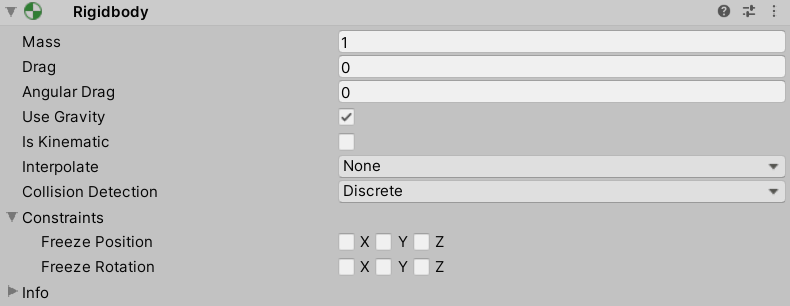
\includegraphics[width=140mm]{rigidbody.png}  
	\caption{Компонент Rigidbody}
	\label{fig:domain:sec_project:rigidbody}
\end{figure}

Настраиваемые свойства \lstinline|Rigidbody|:
\begin{description}
	\item[Mass]	Масса объекта (по умолчанию в килограммах).
	\item[Drag]	Воздушное сопротивление, которое оказывается на объект пока он перемещается под воздействием различных сил. 0 означает отсутствие сопротивления, а бесконечность (infinity) тут же прекращает перемещение объекта.
	\item[Angular Drag]	Воздушное сопротивление, которое оказывается на объект пока он вращается под воздействием силы вращения. 0 означает отсутствие сопротивления. Нельзя остановить вращение объекта путём установки его углового сопротивления (Angular Drag) в бесконечное (infinity) положение.
	\item[Use Gravity]	При включении на объект действует гравитация.
	\item[Is Kinematic]	При включении объект не будет управляться физическим движком, и сможет управляться только при помощи своей трансформации. Полезно при перемещении платформ или если  необходимо анимировать твёрдое тело, которое имеет назначенный HingeJoint.
	\item[Interpolate]	Выбирается одна из опций если была замечена тряска при перемещении твёрдого тела.
	\begin{itemize}
		\item None.	Не применено никакой интерполяции.
		\item Interpolate. Сглаживание транформации основано на трансформации из предыдущего кадра.
		\item Extrapolate. Сглаживание трансформации основано на приблизительной трансформации следующего кадра.
	\end{itemize}
	\item[Collision Detection]	Используется для предотвращения проникновения быстро перемещающихся объектов сквозь другие объекты без определения столкновений.
	\begin{itemize}
		\item Discrete (дискретное). Дискретное обнаружение столкновений со всеми другими коллайдерами в сцене. Другие коллайдеры будут использовать дискретное обнаружение столкновений при тестировании на столкновение с ним. Используется для нормальных столкновений (это значение по умолчанию).
		\item Continuous (непрерывное). Необходимо использовать дискретное обнаружение столкновений с динамическими коллайдерами (с твердым телом) и непрерывное обнаружение столкновений с статическими коллайдерами (без твердого тела). Твердые тела, для которых установлено значение Continuous Dynamic, будут использовать непрерывное обнаружение столкновений при тестировании на столкновение с твердым телом. Другие твердые тела будут использовать дискретное обнаружение столкновений.
		\item Continuous Dynamic (непрерывное динамическое). Используйте непрерывное обнаружение столкновений для объектов GameOject, для которых установлено непрерывное и непрерывное динамическое столкновение. Оно также будет использовать непрерывное обнаружение столкновений со статическими коллайдерами (без твердого тела). Для всех других коллайдеров используется дискретное обнаружение столкновений. Используется для быстро движущихся объектов.
		\item Continuous Speculative (непрерывное спекулятивное). Спекулятивное непрерывное обнаружение столкновений с твердыми телами и коллайдерами. Это также единственный режим обнаружения столкновений, в котором вы можете устанавливать кинематические тела. Этот режим может быть менее дорогим, чем непрерывное обнаружение столкновений.
	\end{itemize}
	\item[Constraints] Ограничения движения твёрдого тела:
	\begin{itemize}
		\item Freeze Position. Выборочно останавливает перемещение твёрдого тела по осям X, Y и Z.
		\item Freeze Rotation. Выборочно останавливает вращение твёрдого тела по осям X, Y и Z.
	\end{itemize}
\end{description}

\subsubsection{Rigidbody2D}~
%cite https://docs.huihoo.com/unity/5.6/Documentation/Manual/class-Rigidbody2D.html

Компонент \lstinline|Rigidbody2D| (Рисунок \ref{fig:domain:sec_project:rigidbody_2d}) помещает объект под контроль физического движка. Многие концепции, знакомые по стандартному компоненту \lstinline|Rigidbody|, переносятся на \lstinline|Rigidbody2D|. Различия в том, что в 2D объекты могут перемещаться только в плоскости XY и могут вращаться только на оси, перпендикулярной этой плоскости.

\begin{figure}[h]
	\noindent\centering
	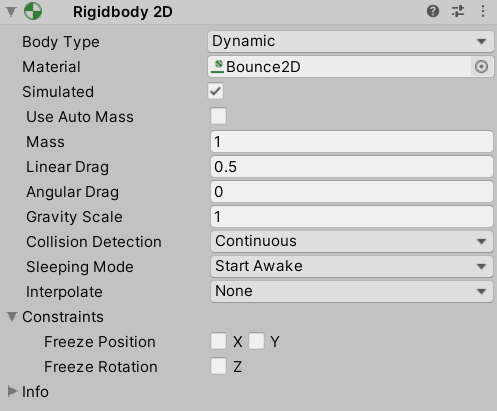
\includegraphics[width=140mm]{rigidbody_2d.png}  
	\caption{Компонент Rigidbody2D}
	\label{fig:domain:sec_project:rigidbody_2d}
\end{figure}

Настраиваемые свойства \lstinline|Rigidbody2D|:
\begin{description}
	\item[Body Type] Есть три варианта для Body Type; каждый определяет фиксированное поведение. Любой Collider2D, прикрепленный к Rigidbody2D, наследует Body Type Rigidbody2D.
	\begin{itemize}
		\item Dynamic. Динамическое твёрдое тело предназначено для движения под симуляцией. Оно обладает полным набором доступных свойств, таких как масса и сопротивление воздуха, и подвержено влиянию силы тяжести. Динамическое тело сталкивается с любым другим типом тела и является наиболее интерактивным из типов телосложения. Это тип тела устанавливается по умолчанию для Rigidbody2D, потому что это наиболее распространенный тип тела для объектов, которые должны двигаться. Это также самый дорогой тип тела из-за его динамичного характера и интерактивности со всем вокруг него. Все свойства Rigidbody2D доступны с этим типом тела.
		\item Kinematic. Кинематическое твёрдое тело разработано для симуляции, но только под явным контролем пользователя. В то время как динамическое твёрдое тело зависит от силы тяжести и силы, кинематическое - нет. По этой причине оно быстрое и требует меньше системных ресурсов, чем динамическое. Кинематическое твёрдое тело разработано для явного перемещения через \lstinline|Rigidbody2D.MovePosition| или \lstinline|Rigidbody2D.MoveRotation|. Необходимо использовать физические методы для обнаружения столкновений и скрипты, чтобы решить, куда и как должно двигаться тело.
		\item Static. Статическое твердое тело разработано так, чтобы вообще не двигаться при симуляции. Если что-то сталкивается с ним, статическое твердое тело ведет себя как неподвижный объект (как будто он имеет бесконечную массу). Это также наименее ресурсоемкий тип тела для использования. Статическое тело сталкивается только с динамическими твёрдыми телами. Столкновение двух статических твёрдых тел не поддерживается, поскольку они не предназначены для перемещения.
	\end{itemize}
	\item[Material] Можно использовать это свойство, чтобы указать общий материал для всех коллайдеров, прикрепленных к конкретному родительскому Rigidbody2D. Collider2D использует свое собственное свойство Material, если оно установлено. Если здесь или в Collider2D не указан материал, по умолчанию используется None (Physics Material 2D). При этом используется материал по умолчанию, который можно установить в окне Physics 2D Settings.
	\item[Simulated] Этот флажок включается, если необходимо, чтобы Rigidbody2D и любые подключенные Collider2D и Joint2D взаимодействовали с физическим моделированием во время выполнения. Если это отключено (флажок снят), эти компоненты не взаимодействуют с симуляцией. Этот флажок установлен по умолчанию.
	\item[Use Auto Mass] Этот флажок устанавливается, если необходимо, чтобы Rigidbody2D автоматически определял массу GameObject из его Collider2D.
	\item[Mass] Определяет массу твердого тела 2D. Заблокировано, если Выбрано «Использовать автоматическую массу».
	\item[Linear Drag] Коэффициент сопротивления, влияющий на позиционное движение.
	\item[Angular Drag] Коэффициент сопротивления, влияющий на вращательное движение.
	\item[Gravity Scale] Коэффициент гравитации. Определяет степень влияния гравитации на GameObject.
	\item[Collision Detection] Определяет, как обнаруживаются столкновения с другими объектами GameObject.
	\item[Sleeping Mode] Спящий режим. Определяет, как GameObject «спит», чтобы сэкономить процессорное время, когда он находится в состоянии покоя.
	\item[Interpolate] Определяет, как движение GameObject интерполируется между обновлениями физики (полезно, когда движение имеет тенденцию к рывкам).
	\item[Constraints] Определяет любые ограничения на движение твёрдого тела.
	\begin{itemize}
		\item Freeze Position. Останавливает перемещение твёрдого тела по осям X и/или Y.
		\item Freeze Rotation. Останавливает вращение твёрдого тела по оси Z.
	\end{itemize}
\end{description}



\subsubsection{Physics Material}~

Физический материал (Рисунок \ref{fig:domain:sec_project:physics_material}) используется для регулировки трения и отскока, возникающего между физическими объектами, когда они сталкиваются.

\begin{figure}[h]
	\noindent\centering
	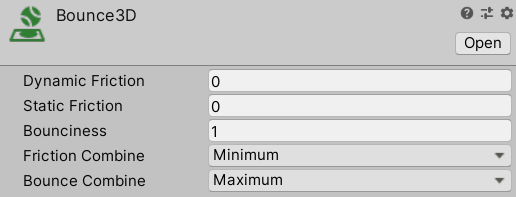
\includegraphics[width=140mm]{physics_material.png}  
	\caption{Компонент Physics Material}
	\label{fig:domain:sec_project:physics_material}
\end{figure}

\begin{description}
	\item[Dynamic Friction]	Трение во время движения. Принимает значения в диапазоне от 0 до 1, где 0 соответствует слабому трению (как на льду), а 1 означает сильное трение, при котором объекту будет сложно двигаться без воздействия внешних сил.
	\item[Static Friction] Трение, использующееся, когда объект лежит на поверхности. Обычно значения бывают в диапазоне от 0 до 1. Значение равное 0 означает отсутствие трения, в то время как значение равное 1 будет означать абсолютное трение (т.е. объектам по такой поверхности будет сложно передвигаться).
	\item[Bounciness] Коэффициент отскока от поверхности (коэффициент восстановления скорости). Значение 0 указывает на отсутствие отскока, а значение 1 указывает на идеальный отскок без потери энергии. Возможны определенные приближения, хотя это может добавить небольшое количество энергии для моделирования.
	\item[Friction Combine]	Как комбинируется между собой трение двух объектов.
	\begin{itemize}
		\item Average. Значения 2 трений усредняются.
		\item Minimum. Из двух значений используется то, что меньше.
		\item Maximum. Из двух значений используется то, что больше.
		\item Multiply. Значения трений умножаются друг на друга.
	\end{itemize}
	\item[Bounce Combine] Как комбинируется упругость двух сталкивающихся объектов. Поддерживает те же режимы, что и Friction Combine.
\end{description}

\subsubsection{Physics Material 2D}~

Физический 2D материал (Рисунок \ref{fig:domain:sec_project:physics_material_2d}) используется для регулировки трения и отскока, возникающего между физическими 2D объектами, когда они сталкиваются.

\begin{figure}[h]
	\noindent\centering
	
\includegraphics[width=140mm]{physics_material_2d.png}  
	\caption{Компонент Physics Material 2D}
	\label{fig:domain:sec_project:physics_material_2d}
\end{figure}

\begin{description}
	\item[Friction] Коэффициент трения для коллайдера.
	\item[Bounciness] Коэффициент отскока от поверхности (коэффициент восстановления скорости). Значение 0 указывает на отсутствие отскока, а значение 1 указывает на идеальный отскок без потери энергии.
\end{description}


\subsection{Проектирование траектории движения двумерных объектов}

\subsubsection{Линейное движение}~

Для начала спроектируем траекторию линейно движущегося объекта на которое не оказывает влияние сила тяжести и не учитываются пересечения с другими объектами. Для рассчёта положения объекта относительно времени воспользуемся формулами \ref{math.position_x} и \ref{math.position_y} с учётом того, что наша скорость постоянна и не изменяется с течением времени, а так же на объект не воздействует гравитационное ускорение ($g = 0$). У игрового объекта, для которого рассчитываем траектрию движения установим Gravity scale = 0.

Для построения траектории воспользуемся методами, описанными в листинге \ref{listing.trajectory_linear}:

\begin{lstlisting}[style=fsharpstyle, caption={Построение траектории линейно движущегося объекта без воздействия силы тяжести и отскоков}, label=listing.trajectory_linear]
List<Vector3> GetTrajectoryPointsLinear(Vector3 startPosition, Vector3 initialVelocity)
{
	Vector3[] segments = new Vector3[segmentsCount];
		
	segments[0] = startPosition;
		
	Vector3 velocity = initialVelocity;
		
	for (int i = 1; i < segmentsCount; i++)
	{
		float segTime = (velocity.sqrMagnitude != 0) ? segmentLength / velocity.magnitude : 0;
		segments[i] = segments[i - 1] + velocity * segTime;
	}
	
	return segments.ToList();
}
\end{lstlisting}

Запустим приложение и видим, что движение объекта совпадает с построенной траекторией (Рисунок \ref{picture.trajectory_linear}).

\begin{figure}[h]
	\noindent\centering
	
\includegraphics[width=140mm]{trajectory_linear.png}  
	\caption{Движение объекта по линейной траектории без воздействия силы тяжести и отскоков}
	\label{picture.trajectory_linear}
\end{figure}

\subsubsection{Гравитация}~

Добавим условие воздейстия на объект силы гравитации. Для рассчёта положения объекта относительно времени воспользуемся формулами \ref{math.position_x} и \ref{math.position_y} с учётом того, что на объект воздействует гравитационное ускорение ($g = 9.81$). Скорость объекта будет изменяться в соответствии с формулами \ref{math.velocity_x} и \ref{math.velocity_y}. У игрового объекта, для которого рассчитываем траектрию движения установим Gravity scale != 0.

Обновлённый код с учётом воздействия гравитации можно увидеть на листинге \ref{listing.trajectory_with_gravity}:

\begin{lstlisting}[style=fsharpstyle, caption={Построение траектории движущегося объекта c учётом гравитации}, label=listing.trajectory_with_gravity]
List<Vector3> GetTrajectoryPointsWithGravity(Vector3 startPosition, Vector3 initialVelocity)
{
	Vector3[] segments = new Vector3[segmentsCount];
	
	segments[0] = startPosition;
	
	Vector3 velocity = initialVelocity;
	
	var gravityScale = objectPrefab.GetComponent<Rigidbody2D>().gravityScale;
	
	for (int i = 1; i < segmentsCount; i++)
	{
		float segTime = (velocity.sqrMagnitude != 0) ? segmentLength / velocity.magnitude : 0;
		segments[i] = segments[i - 1] + velocity * segTime + Physics.gravity * gravityScale * segTime * segTime / 2;
		velocity += Physics.gravity * gravityScale * segTime;
	}
	
	return segments.ToList();
}
\end{lstlisting}

Запустим приложение и видим, что движение объекта совпадает с построенной траекторией (Рисунок \ref{picture.trajectory_with_gravity}).

\begin{figure}[h]
	\noindent\centering
	
\includegraphics[width=140mm]{trajectory_with_gravity.png}  
	\caption{Движение объекта по траектории под воздействием силы тяжести}
	\label{picture.trajectory_with_gravity}
\end{figure}

\subsubsection{Упругий отскок}~

Для проверки пересечения с другими игровыми объектами мы используем статический метод \lstinline|Physics2D.CircleCast|. Он пускает объект в виде круга из указанной точки в указанном направлении на указанное расстояние. Если на этом расстоянии находится какой-либо другой объект, то возвращается объект \lstinline|RaycastHit2D|, содержащий такие данные о столкновении как точка пересечения, нормаль к точке пересечения, расстояние от начальной точки, \lstinline|Collider2D|, \lstinline|Rigidbody2D| и \lstinline|Transform| объекта, с которым произошло перечечение. Для игрового объекта, для которого рассчитываем траекторию движения установим \lstinline|PhysicsMaterial2D| с Bounciness = 1.

Обновлённый код с учётом воздействия гравитации можно увидеть на листинге \ref{listing.trajectory_reflect}:

\begin{lstlisting}[style=fsharpstyle, caption={Построение траектории движущегося объекта c учётом упругих отскоков от других объектов}, label=listing.trajectory_reflect]
List<Vector3> GetTrajectoryPointsReflect(Vector3 startPosition, Vector3 initialVelocity)
{
	Vector3[] segments = new Vector3[segmentsCount];
	
	segments[0] = startPosition;
	
	Vector3 velocity = initialVelocity;
	
	var gravityScale = objectPrefab.GetComponent<Rigidbody2D>().gravityScale;
	
	for (int i = 1; i < segmentsCount; i++)
	{
		float segTime = (velocity.sqrMagnitude != 0) ? segmentLength / velocity.magnitude : 0;
		
		RaycastHit2D  hit = Physics2D.CircleCast(segments[i - 1], 0.5f, velocity, segmentLength);
		if (hit.collider != null && (Vector2)segments[i - 1] != hit.centroid)
		{
			var hitSegTime = hit.distance / velocity.magnitude;
			segments[i] = segments[i - 1] + velocity * hitSegTime + Physics.gravity * gravityScale * hitSegTime * hitSegTime / 2;
			
			velocity += Physics.gravity * gravityScale * hitSegTime;
			velocity = Vector2.Reflect(velocity, hit.normal);
		}
		else
		{
			segments[i] = segments[i - 1] + velocity * segTime + Physics.gravity * gravityScale * segTime * segTime / 2;
			velocity += Physics.gravity * gravityScale * segTime;
		}
	}
	
	return segments.ToList();
}
\end{lstlisting}

Запустим приложение и видим, что движение объекта совпадает с построенной траекторией (Рисунок \ref{picture.trajectory_reflect}).

\begin{figure}[h]
	\noindent\centering
	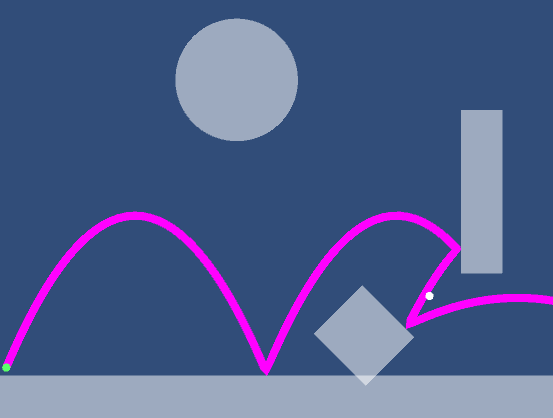
\includegraphics[width=140mm]{trajectory_reflect.png}  
	\caption{Движение объекта c учётом отскоков от других объектов}
	\label{picture.trajectory_reflect}
\end{figure}

\subsubsection{Неупругий отскок}~

Для построения траектории объекта после неупругого столкновения мы воспользуемся формулой \ref{math.bounce}. Учтём, что составляющая скорости объекта коллинеарная нормали изменится в соответствии с коэффициентом восстановления скорости (bounciness) и поменяет направление на противоположное, а касательная составляющая скорости останется неизменной. Для игрового объекта, для которого рассчитываем траектрию движения установим \lstinline|PhysicsMaterial2D| с Bounciness < 1.

Обновлённый код с учётом коэффициента восстановления скорости можно увидеть на листинге \ref{listing.trajectory_bounce}:

\begin{lstlisting}[style=fsharpstyle, caption={Построение траектории движущегося объекта c учётом коэффициента восстановления}, label=listing.trajectory_bounce]
List<Vector3> GetTrajectoryPointsBounce(Vector3 startPosition, Vector3 initialVelocity)
{
	Vector3[] segments = new Vector3[segmentsCount];
	
	segments[0] = startPosition;
	
	Vector3 velocity = initialVelocity;
	
	var bounciness = objectPrefab.sharedMaterial.bounciness;
	var gravityScale = objectPrefab.GetComponent<Rigidbody2D>().gravityScale;
	
	for (int i = 1; i < segmentsCount; i++)
	{
		float segTime = (velocity.sqrMagnitude != 0) ? segmentLength / velocity.magnitude : 0;
		
		RaycastHit2D hit = Physics2D.CircleCast(segments[i - 1], 0.5f, velocity, segmentLength);
		if (hit.collider != null && (Vector2)segments[i - 1] != hit.centroid)
		{
			var hitSegTime = hit.distance / velocity.magnitude;
			segments[i] = segments[i - 1] + velocity * hitSegTime + Physics.gravity * gravityScale * hitSegTime * hitSegTime / 2;
			
			velocity += Physics.gravity * gravityScale * hitSegTime;
			
			var normalVelocity = Vector3.Project(velocity, hit.normal);
			var tangentVelocity = velocity - normalVelocity;
			
			velocity = tangentVelocity - normalVelocity * bounciness;
		}
		else
		{
			segments[i] = segments[i - 1] + velocity * segTime + Physics.gravity * gravityScale * segTime * segTime / 2;
			velocity += Physics.gravity * gravityScale * segTime;
		}
	}
	
	return segments.ToList();
}
\end{lstlisting}

Запустим приложение и видим, что движение объекта совпадает с построенной траекторией (Рисунок \ref{picture.trajectory_bounce}).

\begin{figure}[h]
	\noindent\centering
	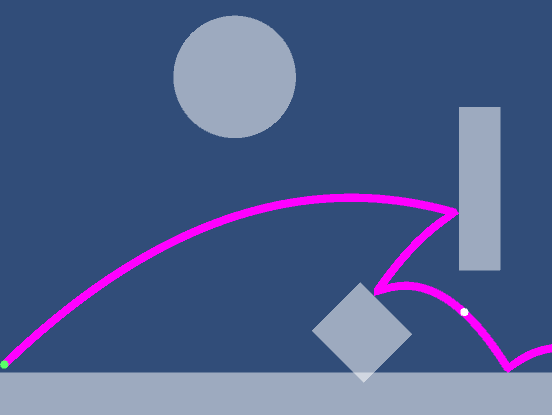
\includegraphics[width=140mm]{trajectory_bounce.png}  
	\caption{Движение объекта c учётом коэффициента восстановления скорости}
	\label{picture.trajectory_bounce}
\end{figure}

\subsubsection{Сопротивление воздуха}~

Сопротивление воздуха воздействующее на тело пока он перемещается для объекта представляется значением \lstinline|Drag|. Можно сказать, что он определяет линейное трение (имеет линейный характер от скорости) и представляет собой значение на которое уменьшается магнитуда скорости в еденицу времени. Метод \lstinline|Mathf.Clamp01(...)| необходим для того чтобы значение скорости в определённый момент не стало отрицательным и объект не двинулся в обратную сторону. Для игрового объекта, для которого рассчитываем траектрию движения установим Drag > 0.

Обновлённый код с учётом сопротивления воздуха можно увидеть на листинге \ref{listing.trajectory_drag}:

\begin{lstlisting}[style=fsharpstyle, caption={Построение траектории движущегося объекта c учётом сопротивления воздуха}, label=listing.trajectory_drag]
List<Vector3> GetTrajectoryPoints(Vector3 startPosition, Vector3 initialVelocity)
{
	Vector3[] segments = new Vector3[segmentsCount];
	
	segments[0] = startPosition;
	
	Vector3 velocity = initialVelocity;
	
	var bounciness = objectPrefab.sharedMaterial.bounciness;
	var drag = objectPrefab.GetComponent<Rigidbody2D>().drag;
	var gravityScale = objectPrefab.GetComponent<Rigidbody2D>().gravityScale;
	
	for (int i = 1; i < segmentsCount; i++)
	{
		float segTime = (velocity.sqrMagnitude != 0) ? segmentLength / velocity.magnitude : 0;
		
		RaycastHit2D hit = Physics2D.CircleCast(segments[i - 1], 0.5f, velocity, segmentLength);
		if (hit.collider != null && (Vector2)segments[i - 1] != hit.centroid)
		{
			var hitSegTime = hit.distance / velocity.magnitude;
			segments[i] = segments[i - 1] + velocity * hitSegTime + Physics.gravity * gravityScale * hitSegTime * hitSegTime / 2;
			
			velocity += Physics.gravity * gravityScale * hitSegTime;
			
			var normalVelocity = Vector3.Project(velocity, hit.normal);
			var tangentVelocity = velocity - normalVelocity;
			
			velocity = tangentVelocity - normalVelocity * bounciness;
			velocity *= Mathf.Clamp01(1f - drag * hitSegTime);
		}
		else
		{
			segments[i] = segments[i - 1] + velocity * segTime + Physics.gravity * gravityScale * segTime * segTime / 2;
			velocity += Physics.gravity * gravityScale * segTime;
			velocity *= Mathf.Clamp01(1f - drag * segTime);
		}
	}
	
	return segments.ToList();
}
\end{lstlisting}

Запустим приложение и видим, что движение объекта совпадает с построенной траекторией (Рисунок \ref{picture.trajectory_drag}).

\begin{figure}[h]
	\noindent\centering
	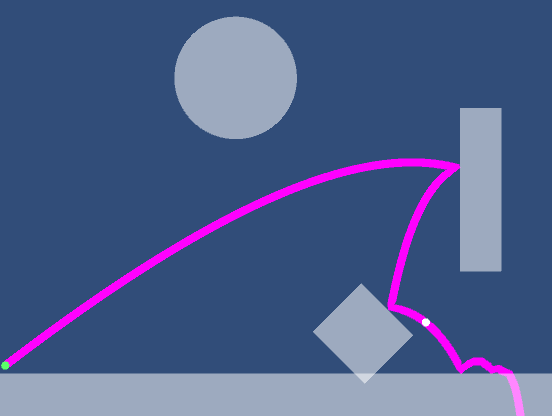
\includegraphics[width=140mm]{trajectory_drag.png}  
	\caption{Движение объекта c учётом сопротивления воздуха}
	\label{picture.trajectory_drag}
\end{figure}

\subsection{Проектирование траектории движения трёхмерных объектов}
В целом построение траектории движения трёхмерного объекта аналогично построению траектории движения двумерного объекта за исключением вычисления вектора скорости после столкновения с другими объектами.

Так для вычисления точки касания и нормали будем использовать метод \lstinline|Physics.SphereCast(...)|. Он пускает объект в виде сферы из указанной точки в указанном направлении на указанное расстояние. Если на этом расстоянии находится какой-либо другой объект, то возвращается объект \lstinline|RaycastHit|, содержащий такие данные о столкновении как точка пересечения, нормаль к точке пересечения, расстояние от начальной точки, \lstinline|Collider|, \lstinline|Rigidbody| и \lstinline|Transform| объекта, с которым произошло перечечение.

Нахождение коэффициента восстановления скорости (отскока) также имеет свои особенности. Когда два тела находятся в контакте, одинаковый эффект отскока применяется к обоим из них в соответствии с выбранным режимом отскока материала (Bounce Combine). Существует особый случай, когда два коллайдера в контакте имеют разные режимы комбинирования. В этом конкретном случае используется функция с наивысшим приоритетом. Порядок приоритетов выглядит следующим образом: Average < Minimum < Multiply < Maximum. Например, если для одного материала установлено значение «Average», а для другого - «Maximum», то используется функция объединения «Maximum», поскольку он имеет более высокий приоритет. Поэтому для рассчёта траектории необходимо учитывать эту особенность материалов.

Код для построения траектории объекта в трёхмерном пространстве можно увидеь на листинге \ref{listing.trajectory_3d}:

\begin{lstlisting}[style=fsharpstyle, caption={Построение траектории трёхмерного движущегося объекта}, label=listing.trajectory_3d]
List<Vector3> GetTrajectoryPoints(Vector3 startPosition, Vector3 initialVelocity)
{
	Vector3[] segments = new Vector3[segmentsCount];
	
	segments[0] = startPosition;
	
	Vector3 velocity = initialVelocity;
	var collider = objectPrefab.GetComponent<Collider>();
	var rigidbody = objectPrefab.GetComponent<Rigidbody>();
	
	var drag = rigidbody.drag;
	var gravityScale = rigidbody.useGravity ? 1 : 0;
	var bounciness = collider.material.bounciness;
	var bounceCombine = collider.material.bounceCombine;
	
	
	for (int i = 1; i < segmentsCount; i++)
	{
		float segTime = (velocity.sqrMagnitude != 0) ? segmentLength / velocity.magnitude : 0;
		
		bool hasHit = Physics.SphereCast(segments[i - 1], 0.5f, velocity, out RaycastHit hit, segmentLength);
		if (hasHit)
		{
			var hitSegTime = hit.distance / velocity.magnitude;
			segments[i] = segments[i - 1] + velocity * hitSegTime + Physics.gravity * gravityScale * hitSegTime * hitSegTime / 2;
			
			velocity += Physics.gravity * gravityScale * hitSegTime;
			
			var normalVelocity = Vector3.Project(velocity, hit.normal);
			var tangentVelocity = velocity - normalVelocity;
			
			var otherBounciness = hit.collider.material.bounciness;
			var otherBounceCombine = hit.collider.material.bounceCombine;
			
			var hitBounceCombine = (PhysicMaterialCombine)Mathf.Max((int)bounceCombine, (int)otherBounceCombine);
			
			var hitBounciness = hitBounceCombine == PhysicMaterialCombine.Average ? (bounciness + otherBounciness) / 2
			: hitBounceCombine == PhysicMaterialCombine.Maximum ? Mathf.Max(bounciness, otherBounciness)
			: hitBounceCombine == PhysicMaterialCombine.Minimum ? Mathf.Min(bounciness, otherBounciness)
			: bounciness * otherBounciness;
			
			velocity = tangentVelocity - normalVelocity * hitBounciness;
			velocity *= Mathf.Clamp01(1f - drag * hitSegTime);
		}
		else
		{
			segments[i] = segments[i - 1] + velocity * segTime + Physics.gravity * gravityScale * segTime * segTime / 2;
			velocity += Physics.gravity * gravityScale * segTime;
			velocity *= Mathf.Clamp01(1f - drag * segTime);
		}
	}
	
	return segments.ToList();
}
\end{lstlisting}

Запустим приложение и видим, что движение объекта совпадает с построенной траекторией (Рисунок \ref{picture.trajectory_3d}).

\begin{figure}[h]
	\noindent\centering
	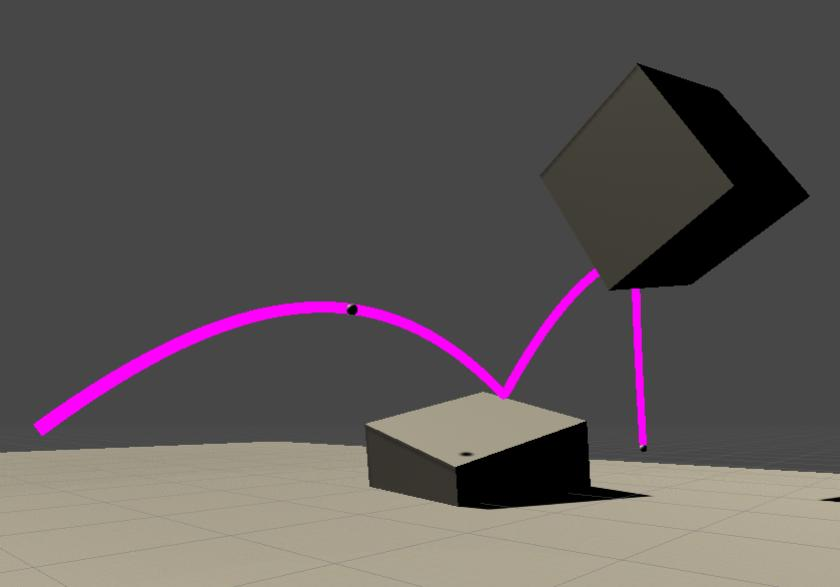
\includegraphics[width=140mm]{trajectory_3d.jpg}  
	\caption{Движение трёхмерного объекта}
	\label{picture.trajectory_3d}
\end{figure}






%\include{sec_ot}

\section{ТЕХНИКО-ЭКОНОМИЧЕСКОЕ ОБОСНОВАНИЕ ПРОГРАММНОГО МОДУЛЯ ДЛЯ РАСЧЕТА ТРАЕКТОРИИ ДВИЖЕНИЯ ОБЪЕКТОВ В ИГРОВЫХ ПРИЛОЖЕНИЯХ}

\subsection{Характеристика проекта}
Разработанный программный модуль представляет собой приложение предназначенное для расчета и построения траектории движения физических тел с использованием игрового движка Unity. 
 
Модуль, написанный с использованием движка Unity позволяет:
\begin{itemize}
	\item Рассчитывать траекторию и имитировать полет объекта из одной точки пространства в другую.
	\item Рассчитывать траекторию и имитировать полёт объекта с учетом большого количества упругих столкновений с другими объектами.
	\item Манипулировать физическими параметрами летящих объектов и полета в общем (скоростью полёта, количеством летящих объектов, размерами объектов, силой трения с другими объектами, гравитацией).
	%\item Хранить данные траектории полёта в локальной и удаленной базе данных.
	%\item Синхронизировать данные между локальной и удаленной базами данных при необходимости.
	%\item Настраивать физические параметры летящих объектов в удаленной базе данных при помощи программного интерфейса.
\end{itemize}

Разработка программного модуля осуществлялась в среде Unity c использованием Unity Editor и Visual Studio.

Полученный модуль может использоваться для построения траектории и имитации движения различных объектов в кроссплатформенных игровых приложениях, построенных в среде Unity. Модуль может быть загружен в Unity Asset Store для продажи другим разработчикам. Модуль не имеет ограничений на используемую платформу и может быть использован на любых платформах поддерживаемых движком Unity. 

Пользователями полученного программного модуля могут являться как отдельные разработчики, так и компании, нуждающиеся в построении траектории движения объектов в пространстве.

Также модуль может быть использован в научных целях для исследования движений различных тел при некоторых заданных параметрах движения и окружающей среды.

Разрабатываемый модуль позволяет уменьшить время, затрачиваемое на разработку приложений, нуждающихся в построении траектории объектов на плоскости и в пространстве.

Модуль имеет самостоятельное значение. Разработка выполняется по договору с компанией BYBN. Личные неимущественные права принадлежат разработчику, а имущественные (исключительные) права переходят компании BYBN (собственнику разработки).

Расчеты ТЭО выполнены на май 2020 года.

\subsection{Расчет прогнозного экономического эффекта от реализации программного средства вычислительной техники}


%\include{sec_final}

% Зачем: Изменение надписи для списка литературы
% Почему: Пункт 2.8.1 Требований по оформлению пояснительной записки.
\renewcommand{\bibsection}{\sectioncentered*{Cписок использованных источников}}
\phantomsection\pagebreak% исправляет нумерацию в документе и исправляет гиперссылки в pdf
\addcontentsline{toc}{section}{Cписок использованных источников}

% Зачем: Печать списка литературы. База данных литературы - файл bibliography_database.bib
\bibliography{bibliography_database}


%\input{annotation} % not part of report

%\input{feedback} % not part of report

%\input{review} % not part of report

% \includepdf позволяет включить в результирующий pdf документ часть другого pdf документа, сделанного
% например не с помощью TeX. Бывает полезно, если какие-то диаграммны нарисованы, например, с помощью 
% Microoft Office и сохранены в pdf.
%\includepdf[pages={-}]{documents_list.pdf}

\end{document}